\documentclass[first=dgreen,second=purple,logo=yellowexc]{aaltoslides}
 
\usepackage{xltxtra,xunicode}
\usepackage{fontspec}
\usepackage{verbatim}
\usepackage{bm}
\usepackage{hyperref}
\usepackage{subfig}
\usepackage{caption}
\usepackage{graphicx}

\usepackage[citestyle=authoryear,backend = biber]{biblatex}
\addbibresource{multiplicative-nerv-ref.bib}
 
\setmainfont[Mapping=tex-text]{Linux Libertine O}
\setmonofont{Consolas}
\setsansfont{Constantia}

%\usepackage[T1]{fontenc}


\title{Multiplicative Update For Fast Optimization Of Information Retrieval Based Neighbor Embedding}
\author{Jaakko Peltonen, Ziyuan Lin}\date{\today}
\institute[ICS]{Department of Information and Computer Science\\
Aalto University, School of Science and Technology}

\DeclareMathOperator*{\argmin}{arg\,min\,}
\DeclareMathOperator*{\argmax}{arg\,max\,}

\begin{document}
%\begin{frame}
%  \titlepage
%\end{frame}

\aaltotitleframe

\begin{frame}{Outline}
\tableofcontents
\end{frame}

\section{Summary}
\begin{frame}{Summary}
\begin{enumerate}
\item \emph{Neighbor Retrieval Visualizer} (NeRV) directly optimizes information retrieval measures which makes it outperform other NLDR methods;
\item We propose a multiplicative update rule for the NeRV;
\item It's fast and preserving good visual quality.
\end{enumerate}
\end{frame}

\section{Neighbor retrieval visualizer}
\begin{frame}{Neighbor retrieval visualizer (NeRV)}
NeRV minimizes two categories of errors: \emph{false neighbors} and \emph{misses}, and establishes connections between the errors and KL-divergences (\cite{venna10jmlr})
\begin{align*}
\{y^*_{ij}\}=&\argmin_{\{y_{ij}\}}\sum_i\sum_{j\ne i}\lambda p_{ij}\log\frac{p_{ij}}{q_{ij}}+(1-\lambda)q_{ij}\log\frac{q_{ij}}{p_{ij}}\\
=&\argmin_{\{y_{ij}\}}\sum_i\lambda KL(P_i\|Q_i)+(1-\lambda)KL(Q_i\|P_i)
\end{align*}
\end{frame}


\begin{frame}{Errors in visual information retrieval}
\begin{figure}
\centering
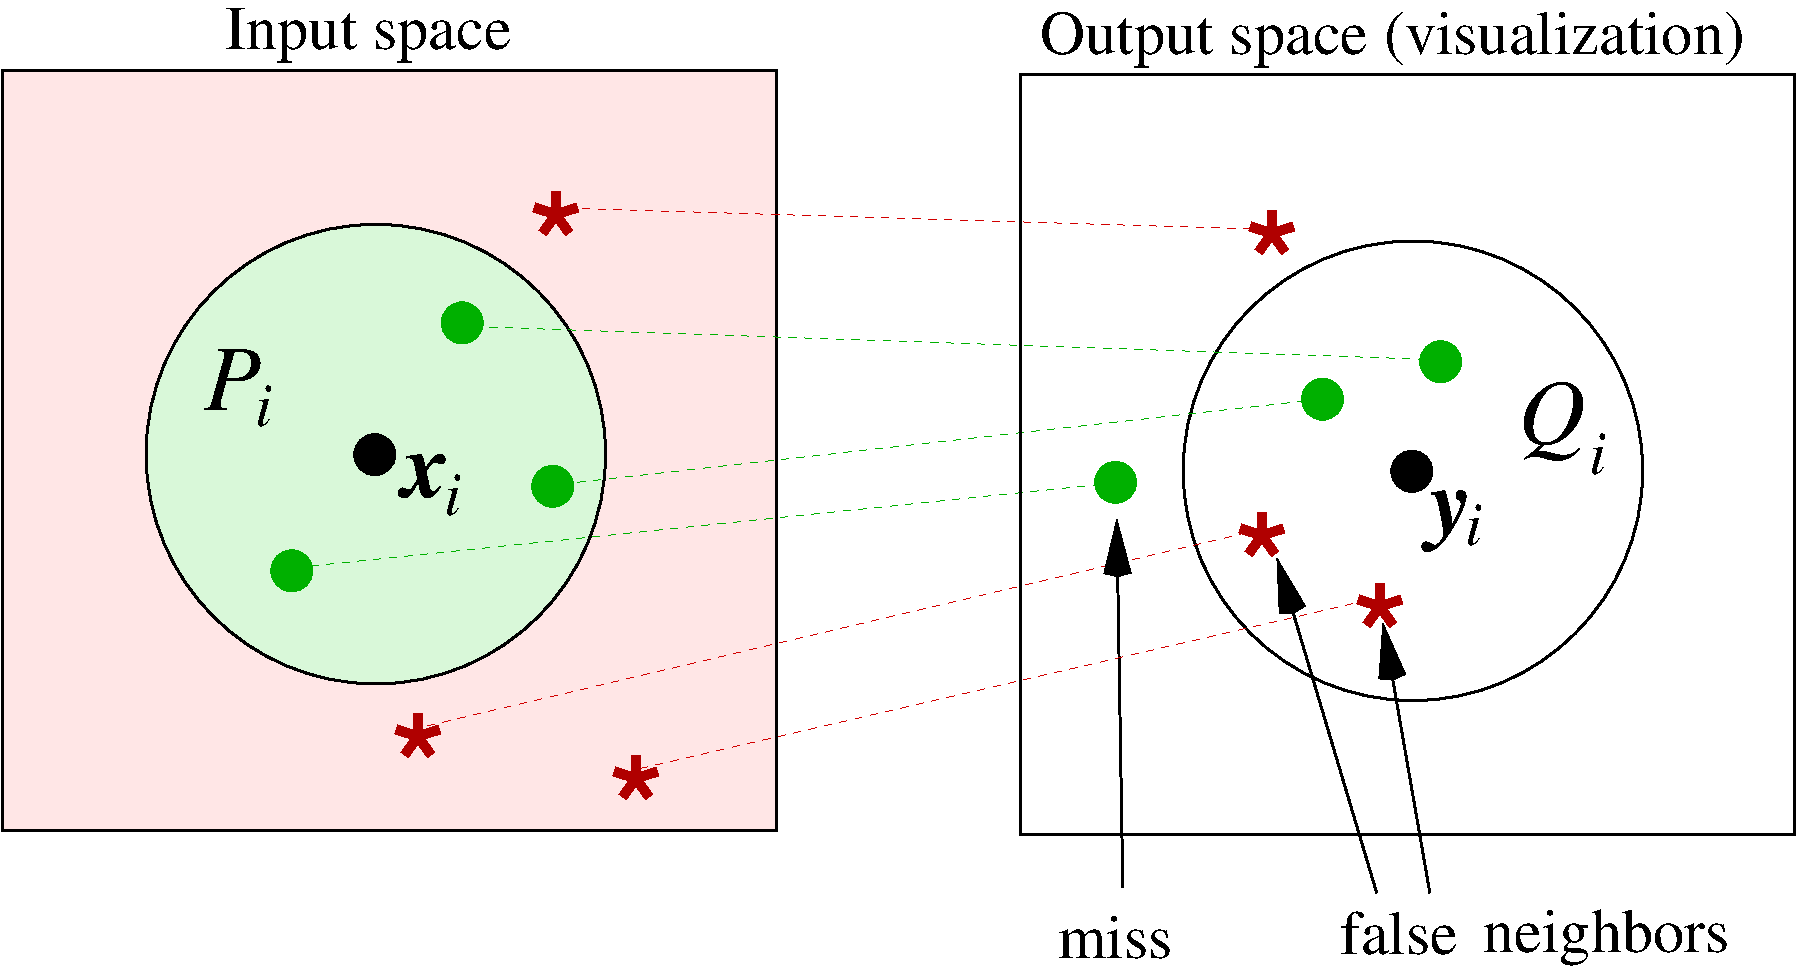
\includegraphics[width=\textwidth]{figures/retrieval_illustration.pdf}
\caption{\footnotesize{Misses are true neighbors that are not neighbors on the display; false neighbors are neighbors on the display that are not true neighbors.}}
\end{figure}
\end{frame}


\begin{frame}{Illustration of NeRV}
\begin{figure}
\begin{columns}
\begin{column}{0.65\textwidth}
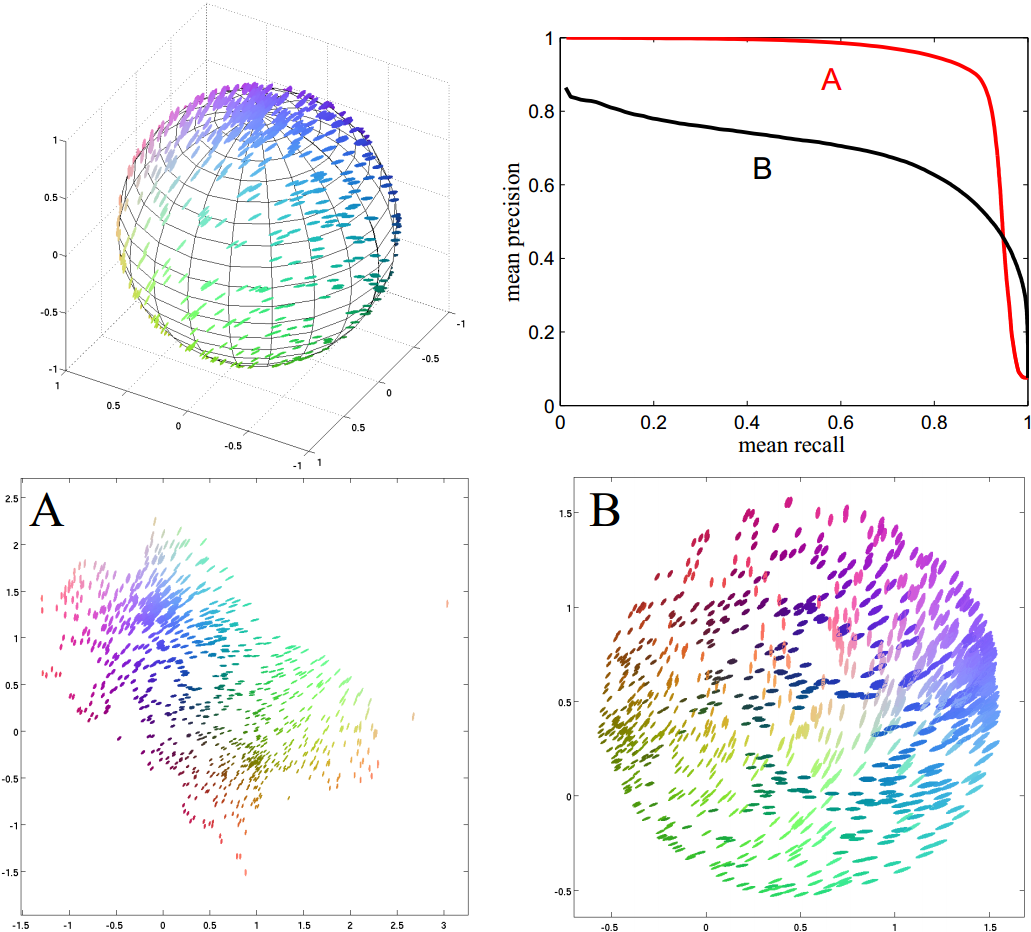
\includegraphics[width=\textwidth]{figures/demo.png}
\end{column}
\begin{column}{0.3\textwidth}
\caption{\scriptsize{Results of NeRV for a toy data set. \textbf{A} minimizes false neighbors (or emphasizes \emph{precision}) while \textbf{B} minimized misses (or emphasizes \emph{recall}). Top right shows the mean precision-mean recall curves as a function of the output neighborhood size $k$.}}
\end{column}
\end{columns}
\end{figure}
\end{frame}

\section{How to make it fast}
\begin{frame}{To speed up NeRV}
\begin{itemize}
\item The original gradient descent based optimization is too slow for some cases, particular when involving user interaction (\cite{peltonen13eurovis})
\item Quad-tree based acceleration: \cite{yang13icml}, \cite{vandermaaten13iclr}
\item Problems: have to assume the neighborhood distribution $p_{ij}$ to be sparse
\end{itemize}
\end{frame}

\begin{frame}{Our method}
Instead of the usual additive update rule
\[
z^{(t+1)}_{id}=z^{(t)}_{id}-\alpha_{id} \nabla_{id} \mathcal{J}(z^{(t)})\;,
\]
we derive the \emph{multiplicative} update rule which is similar to (\cite{yang10mlsp}):
\[
z^{(t+1)}_{id}=z^{(t)}_{id}\frac{\nabla^-_{id} \mathcal{J}(z^{(t)})}{\nabla^+_{id} \mathcal{J}(z^{(t)})}\;,
\]
where
\begin{align*}
z^{(t)}_{id}:&\mbox{ the $(i,d)$-th parameter at the $t$-th iteration;}\\
\mathcal{J}:&\mbox{ the cost function;}\\
\nabla_{id}:&\mbox{ the $(i,d)$-th component of the gradient;}\\
\nabla_{id}^+,\nabla_{id}^-:&\mbox{ satisfy }\nabla_{id}\mathcal{J}=\nabla_{id}^+\mathcal{J}-\nabla_{id}^-\mathcal{J}\mbox{ and }\nabla_{id}^+\mathcal{J},\nabla_{id}^-\mathcal{J}\ge 0
\end{align*}
\end{frame}

\begin{frame}{Connections with additive update}
\begin{enumerate}
\item $\nabla_{id}\mathcal{J}(z_{id})=0 \Longrightarrow \nabla_{id}^+\mathcal{J}(z_{id})=\nabla_{id}^-\mathcal{J}(z_{id})$;
\item
\[
\left.
\begin{aligned}
z^{(t+1)}_{id} =& z^{(t)}_{id}-\alpha_{id} \nabla_{id} \mathcal{J}(z^{(t)})\\
\alpha_{id} =& \frac{z_{id}^{(t)}}{\nabla_{id}^+\mathcal{J}(z_{id}^{(t)})}
\end{aligned}
\right\}\Longrightarrow z^{(t+1)}_{id}=z^{(t)}_{id}\frac{\nabla^-_{id} \mathcal{J}(z^{(t)})}{\nabla^+_{id} \mathcal{J}(z^{(t)})}
\]
\end{enumerate}
Benefit: no need to tune the learning rate $\alpha_{id}$, without changing the "stationary condition".
\end{frame}


\begin{frame}{Multiplicative NeRV in detail}
\begin{enumerate}
\item Re-parameterize using $z_{id}=\exp(y_{id})$ to preserve the sign;
\item Introduce the notations below
\begin{align*}
KL_{ij}=&\frac{1-\lambda}{\sigma_i^2}q_{j|i}D_{KL}(q_i,p_i)\;,\;\;kl_{ij}=\frac{1-\lambda}{\sigma_i^2}q_{j|i}\log\frac{q_{j|i}}{p_{j|i}}\\
P_{ij}=&\frac{\lambda p_{j|i}}{\sigma_i^2}\;,\;\;Q_{ij}=\frac{\lambda q_{j|i}}{\sigma_i^2} \;.
\end{align*}
\end{enumerate}
Interpretations:
\begin{itemize}
\item 
$KL_{ij}-kl_{ij}>0 \Longrightarrow q_{j|i}D_{KL}(q_i,p_i)>q_{j|i}\log\frac{q_{j|i}}{p_{j|i}}$, which means for query point $i$, neighbor $j$ contributed greater to the total false neighbor cost.

\end{itemize}
\end{frame}


\begin{frame}{Multiplicative NeRV in detail}
\begin{enumerate}
\item Re-parameterize using $z_{id}=\exp(y_{id})$ to preserve the sign
\item Introduce the notations below
\begin{align*}
KL_{ij}=&\frac{1-\lambda}{\sigma_i^2}q_{j|i}D_{KL}(q_i,p_i)\;,\;\;kl_{ij}=\frac{1-\lambda}{\sigma_i^2}q_{j|i}\log\frac{q_{j|i}}{p_{j|i}}\\
P_{ij}=&\frac{\lambda p_{j|i}}{\sigma_i^2}\;,\;\;Q_{ij}=\frac{\lambda q_{j|i}}{\sigma_i^2} \;.
\end{align*}
\end{enumerate}

Interpretations:
\begin{itemize}
\item $P_{ij}-Q_{ij}>0 \Longrightarrow p_{j|i}>q_{j|i}$, which means neighbor $j$ is missed for point $i$.

\end{itemize}
\end{frame}


\begin{frame}{Multiplicative NeRV in detail}
We calculated the update as
\[
z_{id}^{(t+1)}=z_{id}^{(t)} \frac{\sum_{j\ne i}A_{ij}^+Y^{d-}_{ij}+A_{ij}^-Y^{d+}_{ij}}{\sum_{j\ne i}A_{ij}^+Y^{d+}_{ij}+A^-_{ij}Y^{d-}_{ij}}
\]
where
\begin{align*}
A_{ij}^+=&(KL_{ij}-kl_{ij})^++(P_{ij}-Q_{ij})^+ +(KL_{ji}-kl_{ji})^++(P_{ji}-Q_{ji})^+ \;,\\
A_{ij}^-=&(KL_{ij}-kl_{ij})^-+(P_{ij}-Q_{ij})^- +(KL_{ji}-kl_{ji})^-+(P_{ji}-Q_{ji})^- \;,\\
Y^{d+}_{ij}=&\left(y_{id}^++y_{jd}^-\right)\;,\;\;\;
Y^{d-}_{ij}=\left(y_{id}^-+y_{jd}^+\right)
\end{align*}
Roughly, The multiplicative update then pushes $y_{id}$ away from the worst false neighbors of $i$ and towards missed neighbors.
\end{frame}

\section{Experiments}
\begin{frame}{Experiments: results on different data sets}
\begin{figure}[!htb]
\captionsetup[subfigure]{labelformat=empty}
\centering
\begin{tabular}{cc}
\subfloat[]{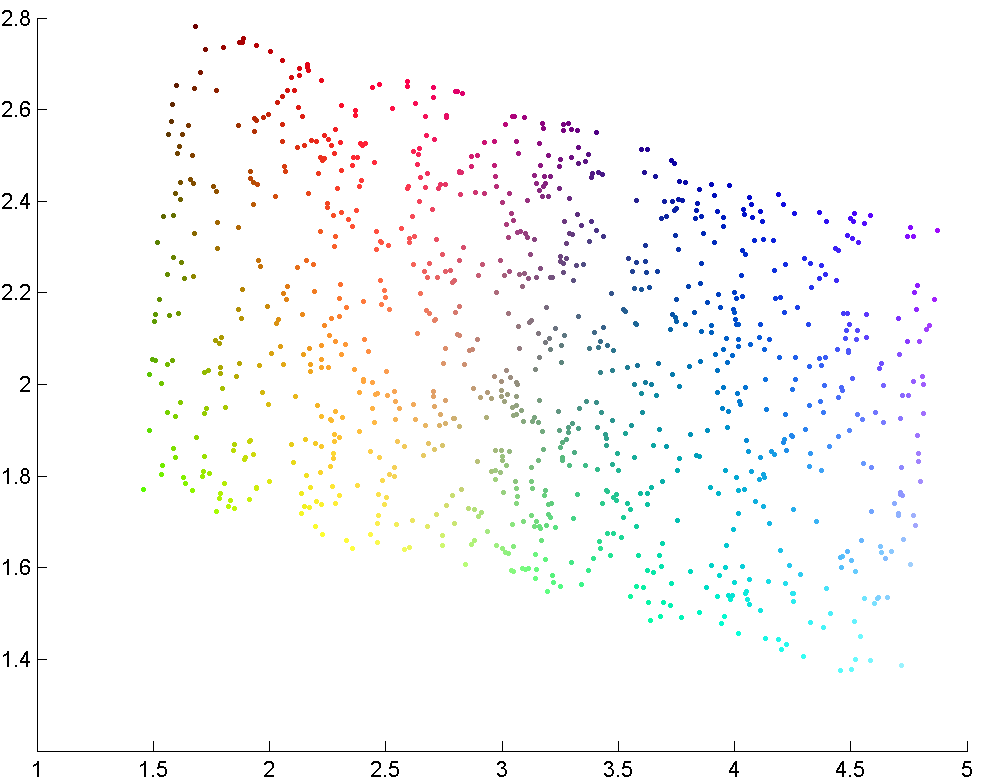
\includegraphics[height=0.5\textheight]{figures/s-data-0-nerv-0_1.pdf}} & 
\subfloat[]{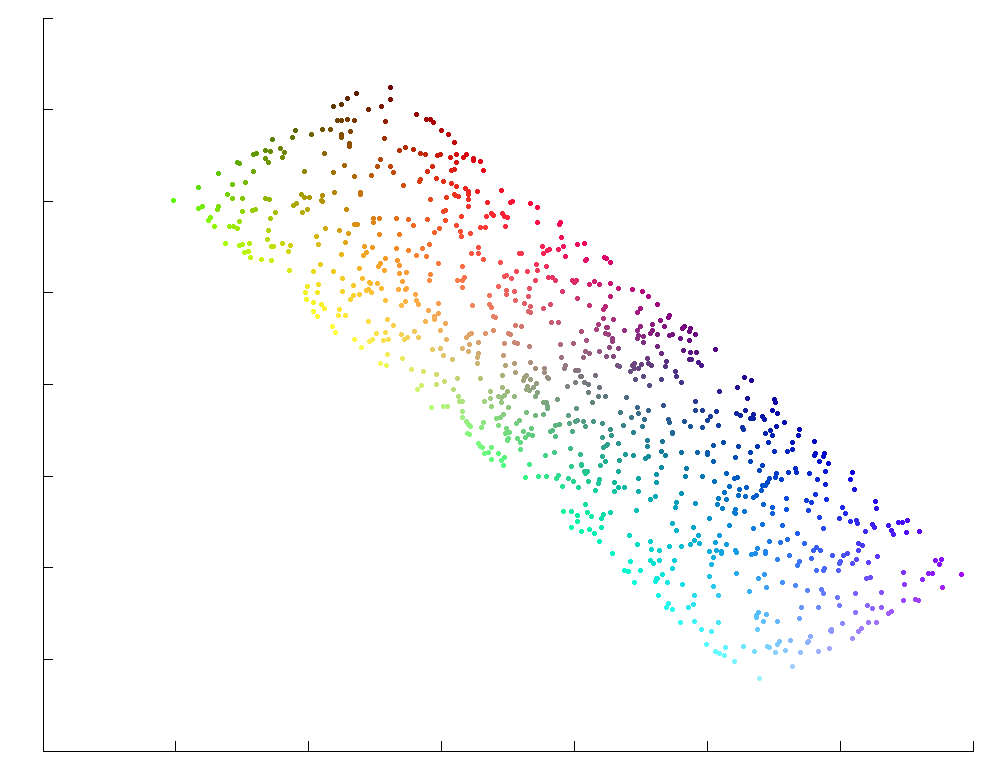
\includegraphics[height=0.5\textheight]{figures/s-data-0-original-nerv-0_1.pdf}}\\
\end{tabular}
\caption{Results of Plain S-curve, multiplicative vs. additive. Colors correspond to original 3D coordinates.}
\end{figure}
\end{frame}


\begin{frame}{Experiments: results on different data sets}
\begin{figure}[!htb]
\captionsetup[subfigure]{labelformat=empty}
\centering
\begin{tabular}{cc}
\subfloat[]{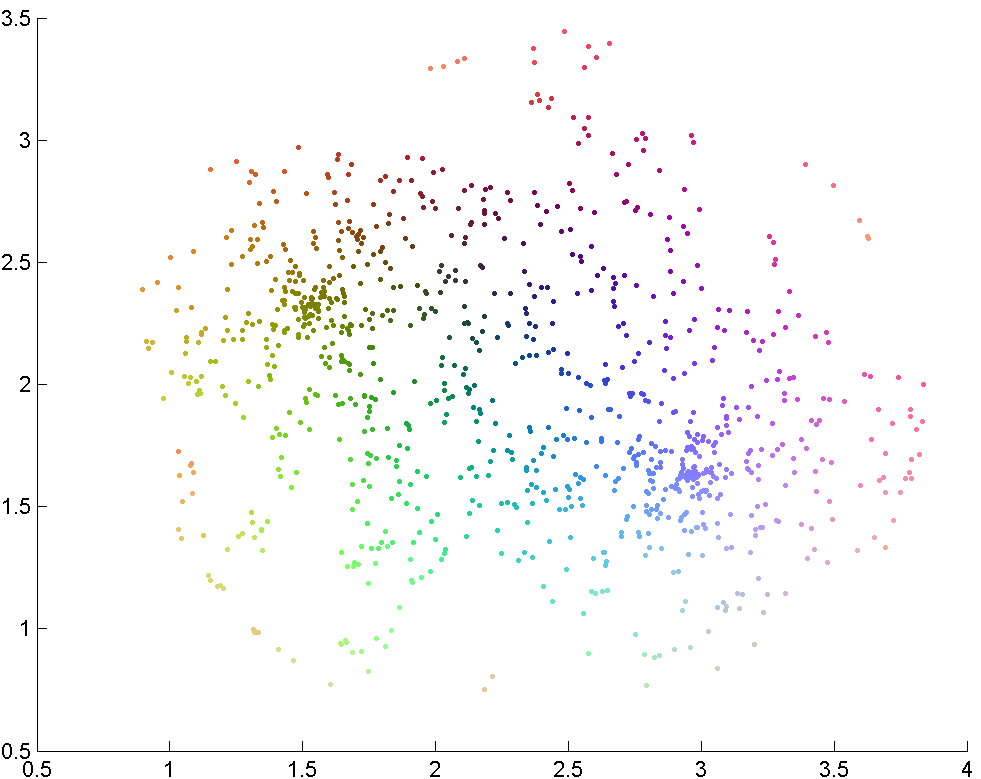
\includegraphics[height=0.5\textheight]{figures/sphere-nerv-0_1.pdf}} &
\subfloat[]{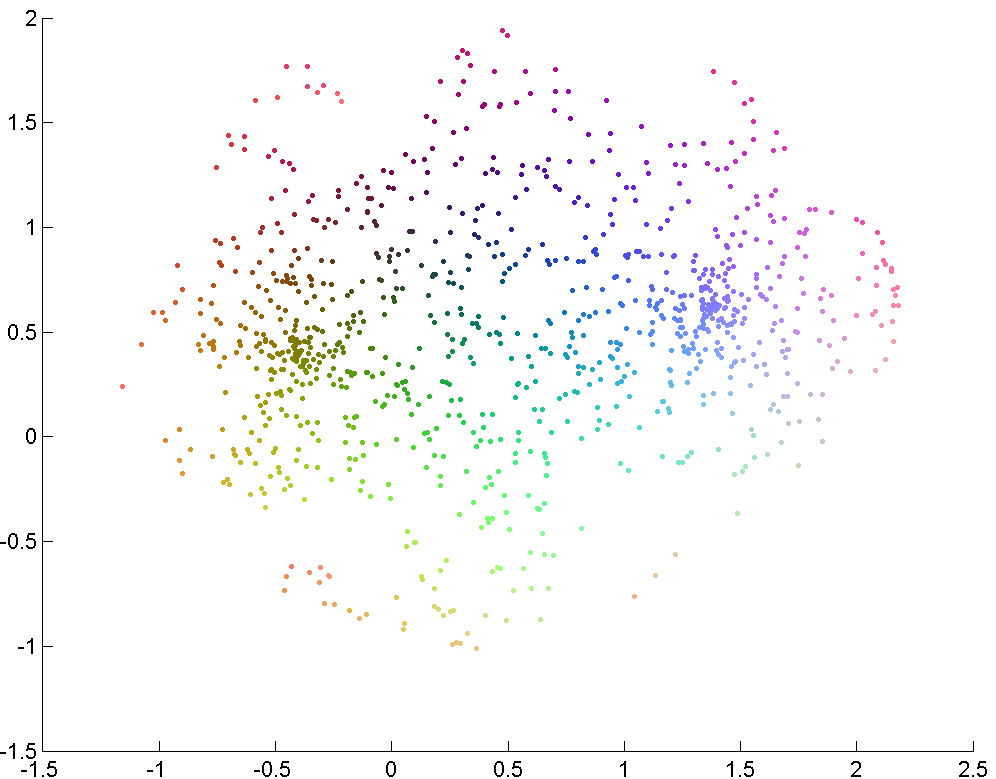
\includegraphics[height=0.5\textheight]{figures/sphere-original-nerv-0_1.pdf}}
\end{tabular}
\caption{Results of Sphere, multiplicative vs. additive. Colors correspond to original 3D coordinates.}
\end{figure}
\end{frame}


\begin{frame}{Experiments: results on different data sets}
\begin{figure}[!htb]
\captionsetup[subfigure]{labelformat=empty}
\centering
\begin{tabular}{cc}
\subfloat[]{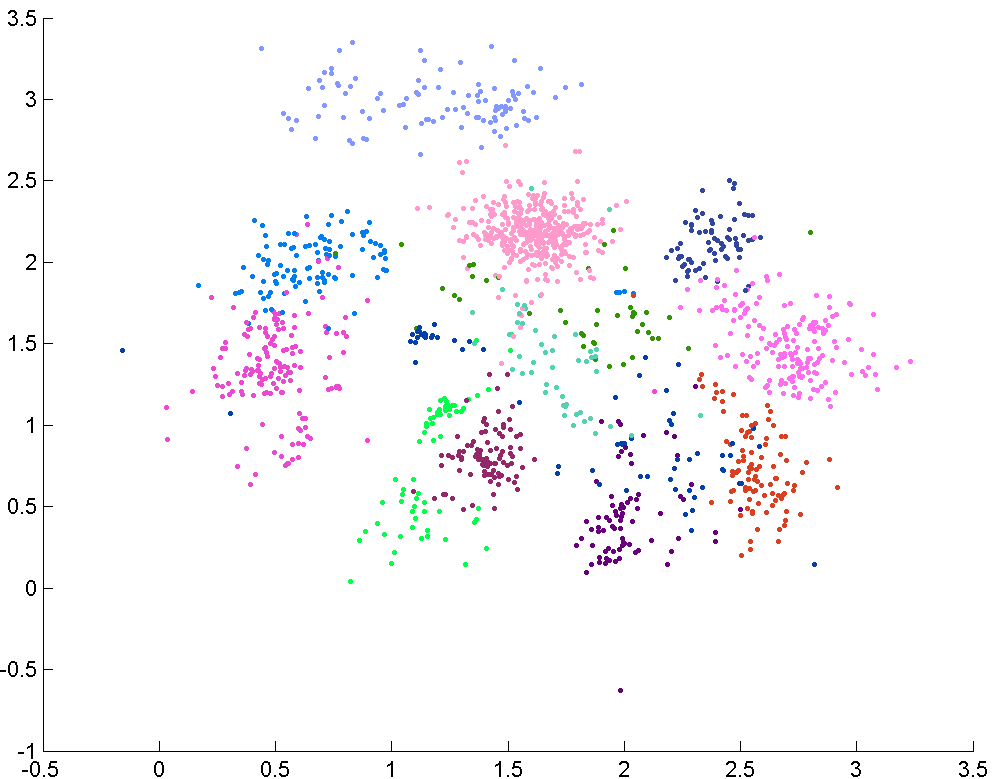
\includegraphics[height=0.5\textheight]{figures/lvqdata-nerv-0_1.pdf}} &
\subfloat[]{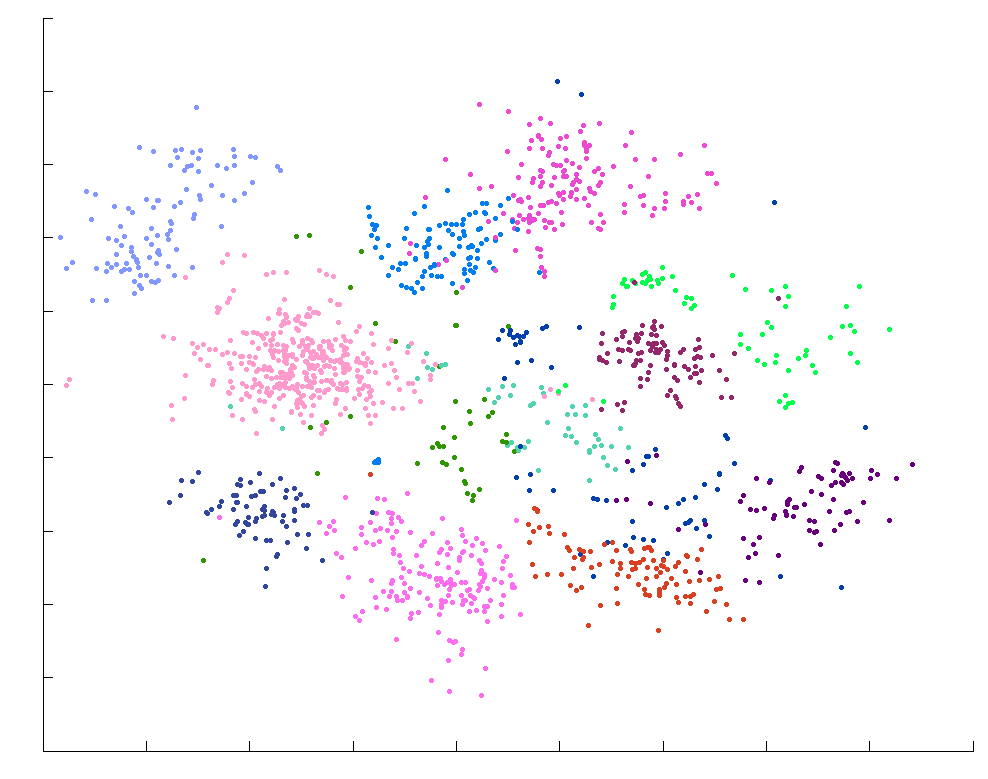
\includegraphics[height=0.5\textheight]{figures/lvqdata-original-nerv-0_1.pdf}}
\end{tabular}
\caption{Results of Phoneme, multiplicative vs. additive. Colors correspond to class labels of data points.}
\end{figure}
\end{frame}


\begin{frame}{Experiments: results on different data sets}
\begin{figure}[!htb]
\captionsetup[subfigure]{labelformat=empty}
\centering
\begin{tabular}{cc}
\subfloat[]{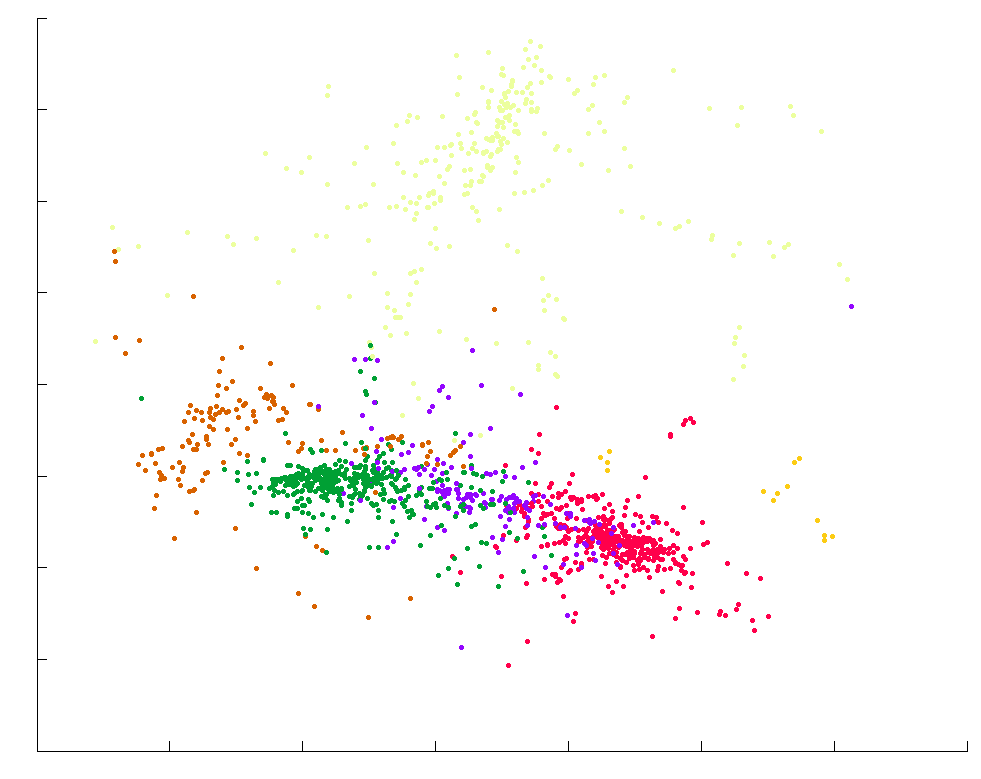
\includegraphics[height=0.5\textheight]{figures/landsat-nerv-0_1.pdf}} &
\subfloat[]{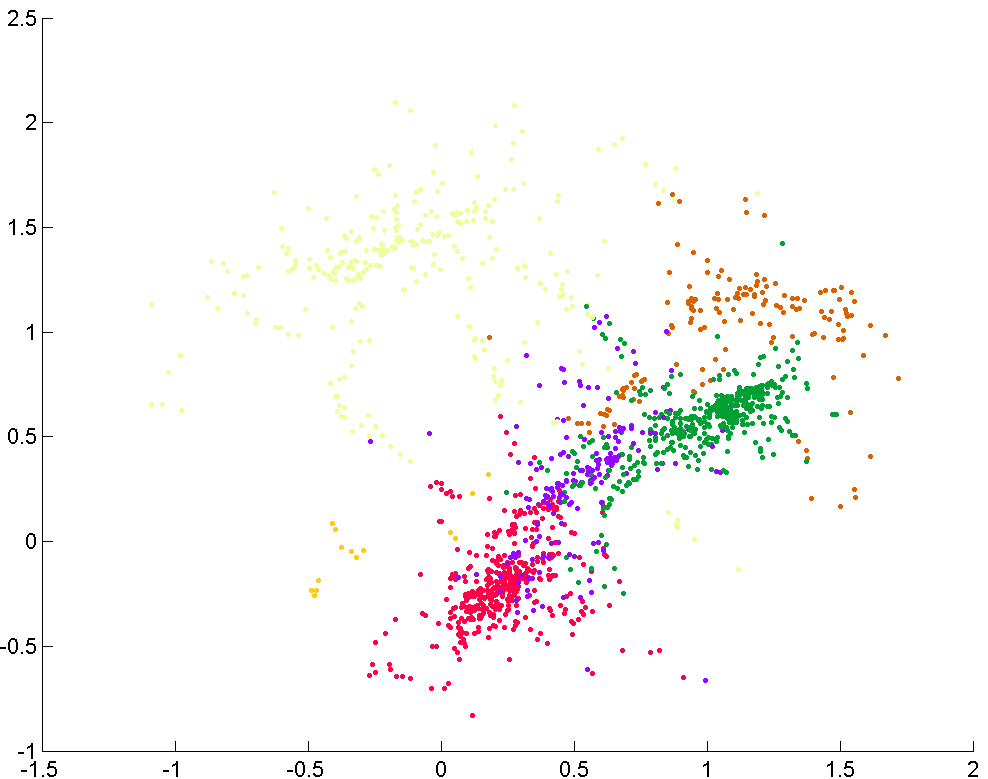
\includegraphics[height=0.5\textheight]{figures/landsat-original-nerv-0_1.pdf}}
\end{tabular}
\caption{Results of Landsat, multiplicative vs. additive. Colors correspond to class labels of data points.}
\end{figure}
\end{frame}


\begin{frame}{Experiments: results on different data sets}
\begin{figure}[!htb]
\captionsetup[subfigure]{labelformat=empty}
\centering
\begin{tabular}{cc}
\subfloat[]{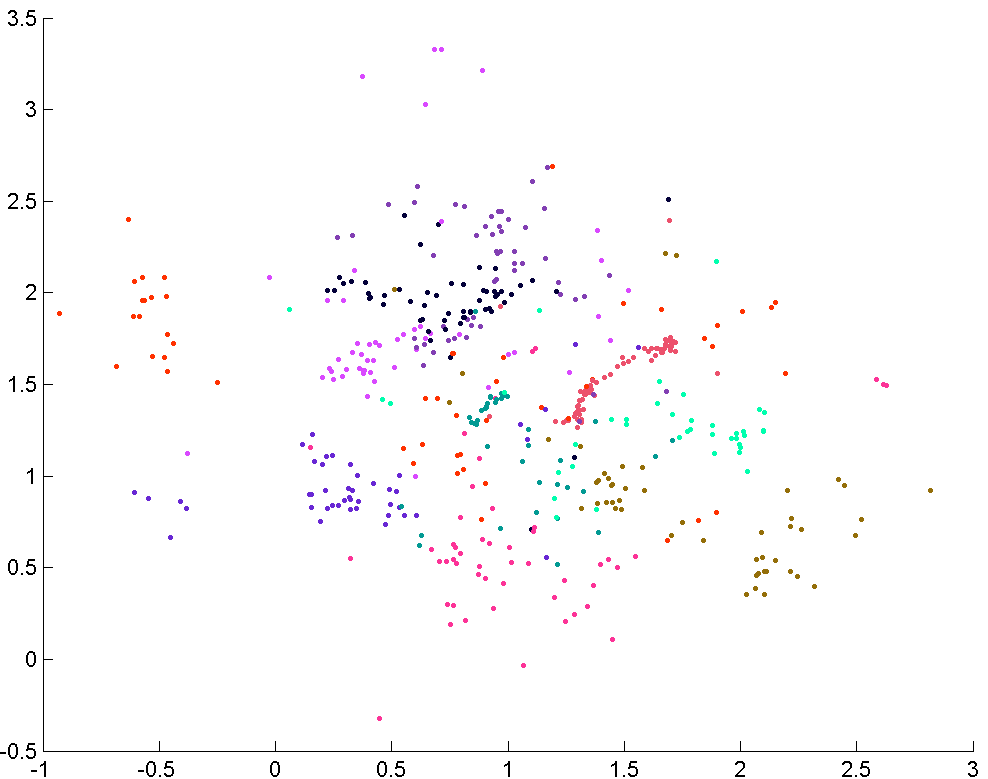
\includegraphics[height=0.5\textheight]{figures/MNIST-500-nerv-0_1.pdf}} &
\subfloat[]{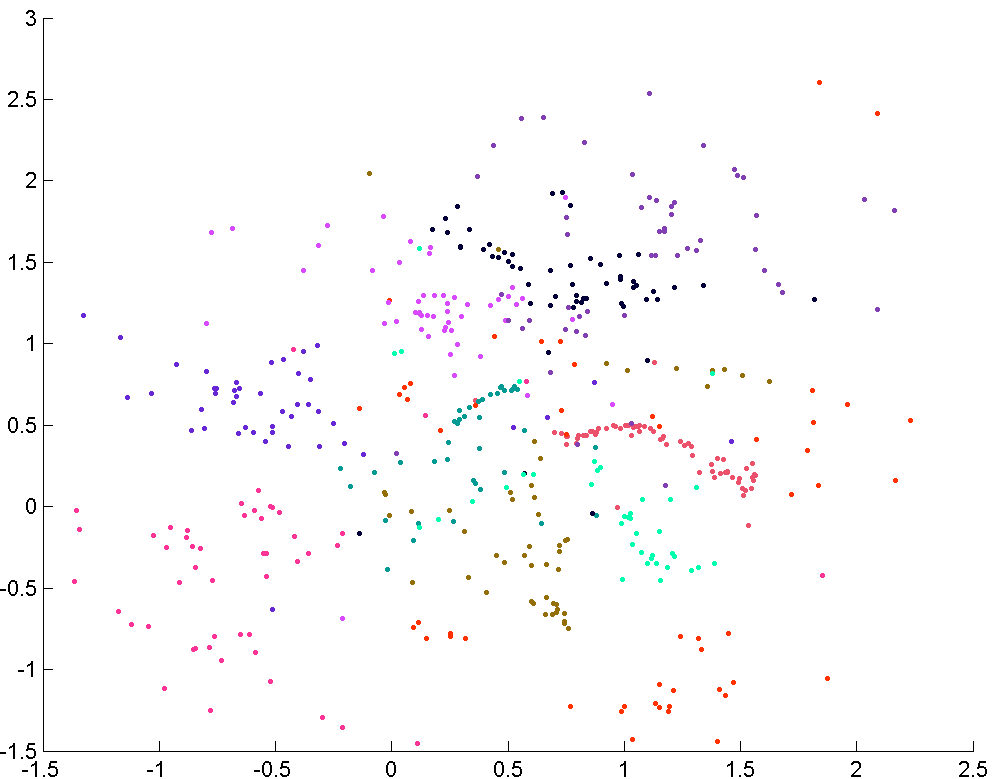
\includegraphics[height=0.5\textheight]{figures/MNIST-500-original-nerv-0_1.pdf}}
\end{tabular}
\caption{Results of MNIST, multiplicative vs. additive. Colors correspond to class labels of data points.}
\end{figure}
\end{frame}


\begin{frame}{Experiments: results on different data sets}
\begin{figure}[!htb]
\captionsetup[subfigure]{labelformat=empty}
\centering
\begin{tabular}{cc}
\subfloat[]{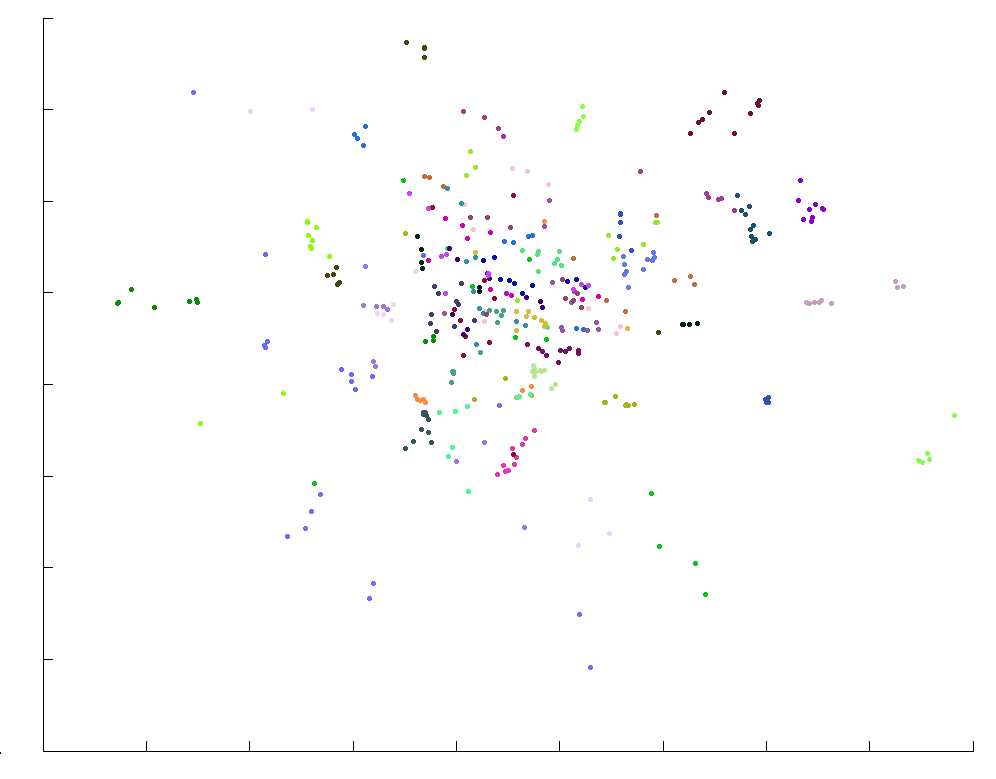
\includegraphics[height=0.5\textheight]{figures/olivettifaces_dist-nerv-0_1.pdf}} &
\subfloat[]{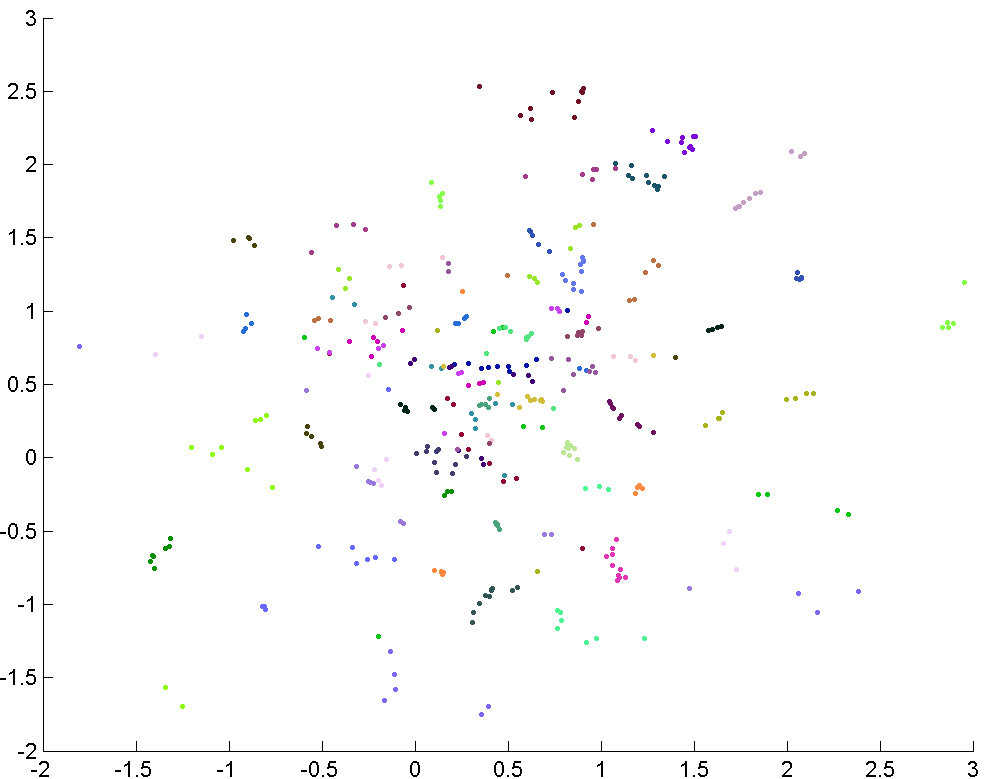
\includegraphics[height=0.5\textheight]{figures/olivettifaces_dist-original-nerv-0_1.pdf}}
\end{tabular}
\caption{Results of olivetti Faces, multiplicative vs. additive. Colors correspond to class labels of data points.}
\end{figure}
\end{frame}


\begin{frame}{Experiments: performance}
\begin{figure}[!htb]
\captionsetup[subfigure]{labelformat=empty}
\centering
\begin{tabular}{cc}
\subfloat[]{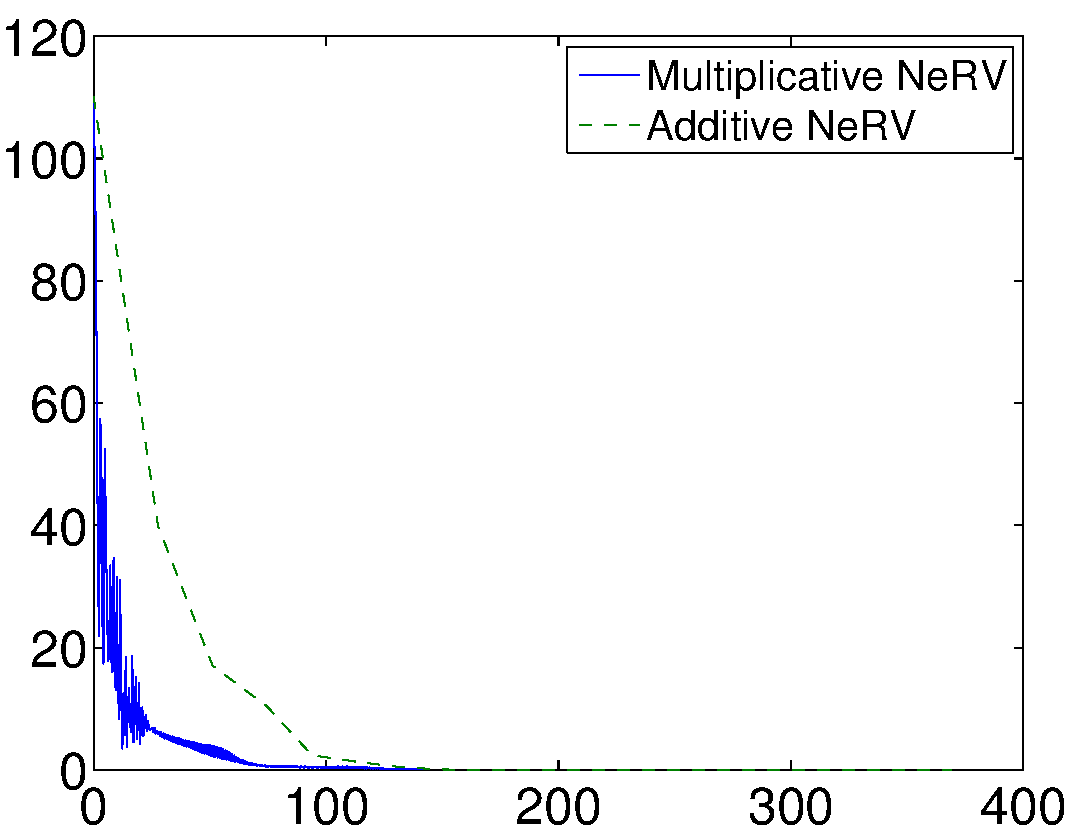
\includegraphics[width=0.5\textwidth]{figures/secs_cost_s-data-0.pdf}} &
\subfloat[]{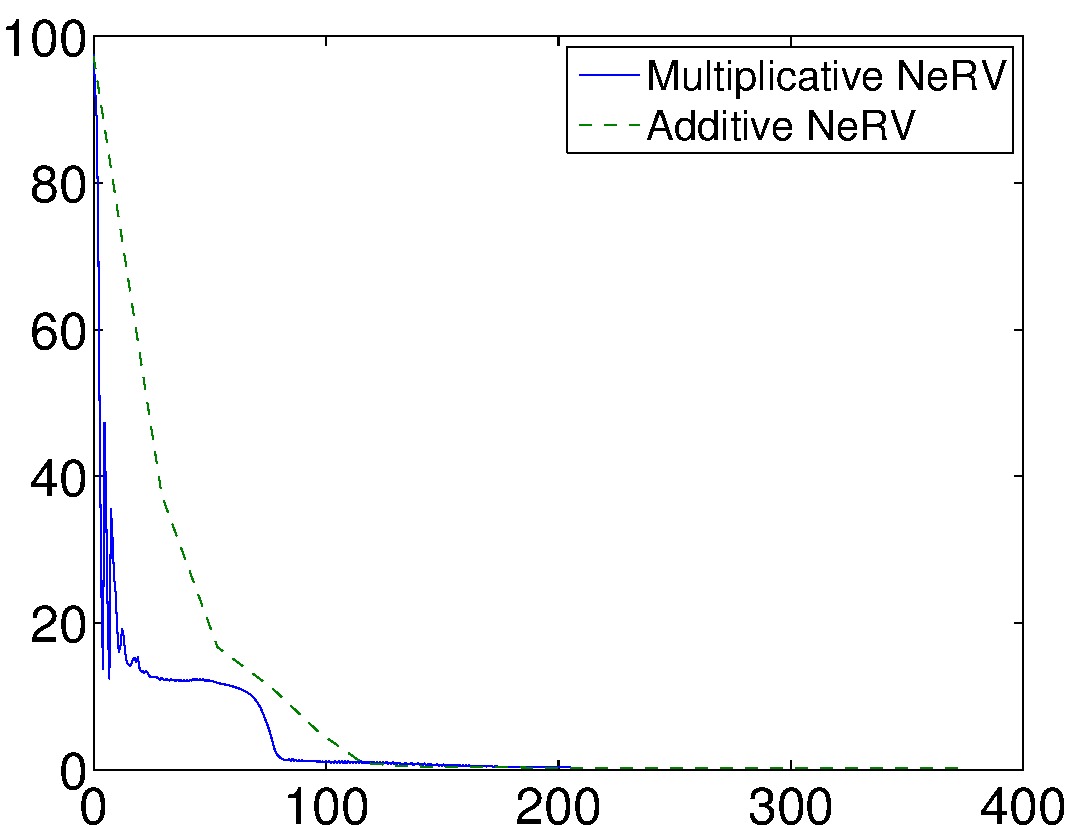
\includegraphics[width=0.5\textwidth]{figures/secs_cost_sphere.pdf}} 
\end{tabular}
\caption{Graphs of running time vs. information retrieval performance (NeRV's cost, the lower the better). Data sets: Plain S-curve and Sphere.}
\end{figure}
\end{frame}


\begin{frame}{Experiments: performance}
\begin{figure}[!htb]
\captionsetup[subfigure]{labelformat=empty}
\centering
\begin{tabular}{cc}
\subfloat[]{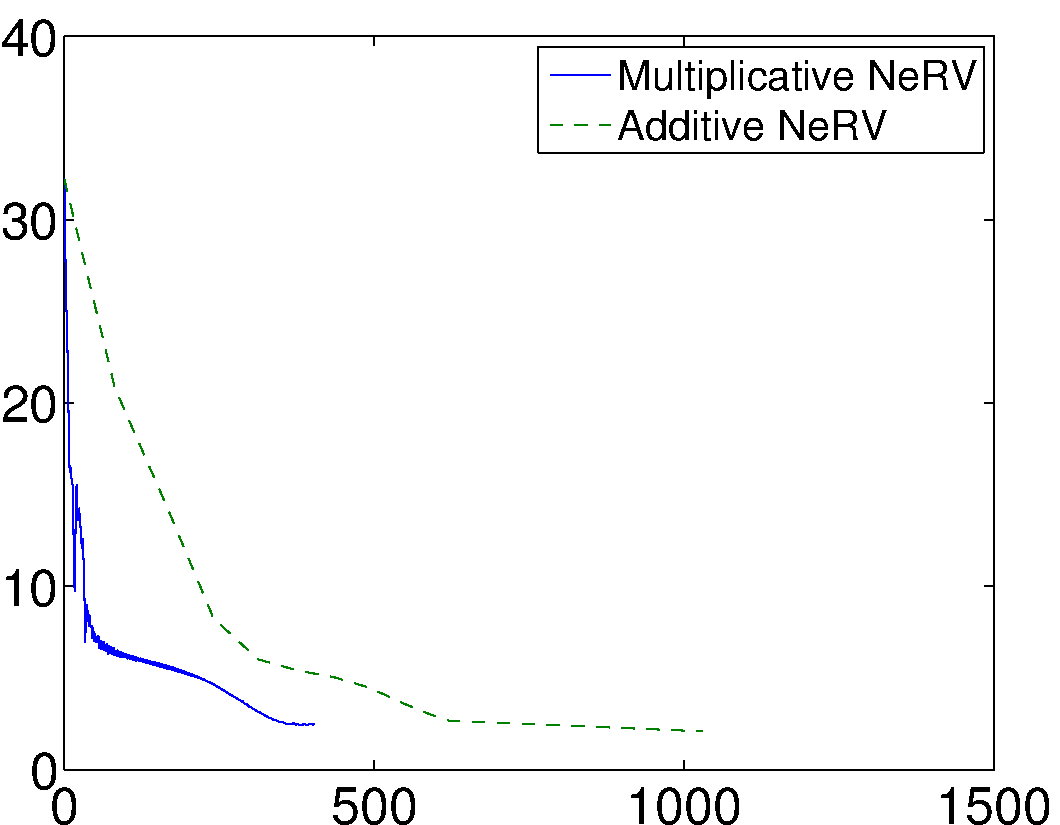
\includegraphics[width=0.5\textwidth]{figures/secs_cost_lvqdata.pdf}} &
\subfloat[]{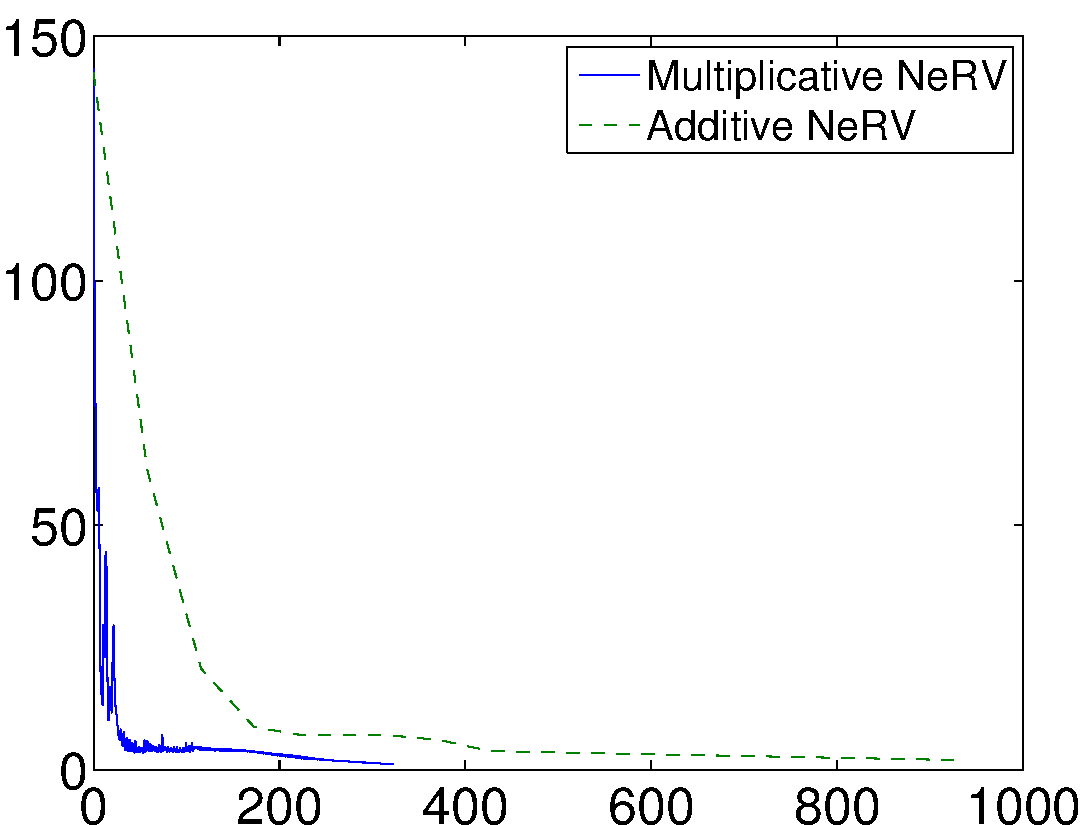
\includegraphics[width=0.5\textwidth]{figures/secs_cost_landsat.pdf}} 
\end{tabular}
\caption{Graphs of running time vs. information retrieval performance (NeRV's cost, the lower the better). Data sets: Phoneme and Landsat.}
\end{figure}
\end{frame}


\begin{frame}{Experiments: performance}
\begin{figure}[!htb]
\captionsetup[subfigure]{labelformat=empty}
\centering
\begin{tabular}{cc}
\subfloat[]{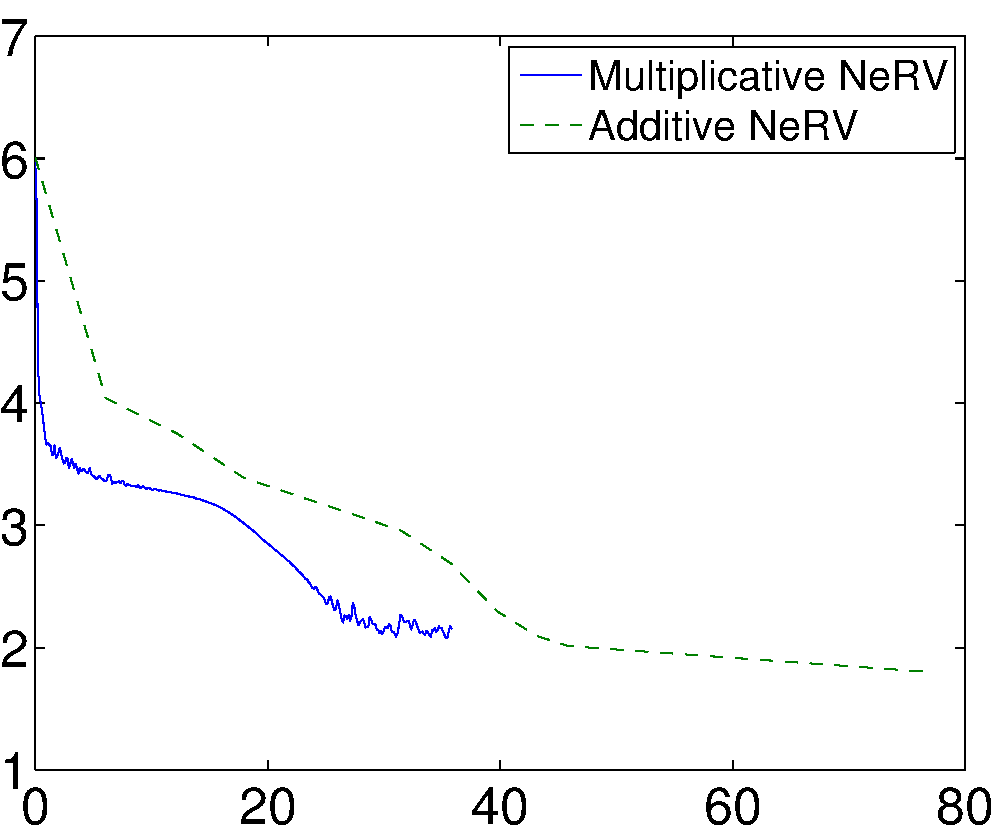
\includegraphics[width=0.5\textwidth]{figures/secs_cost_MNIST-500.pdf}} &
\subfloat[]{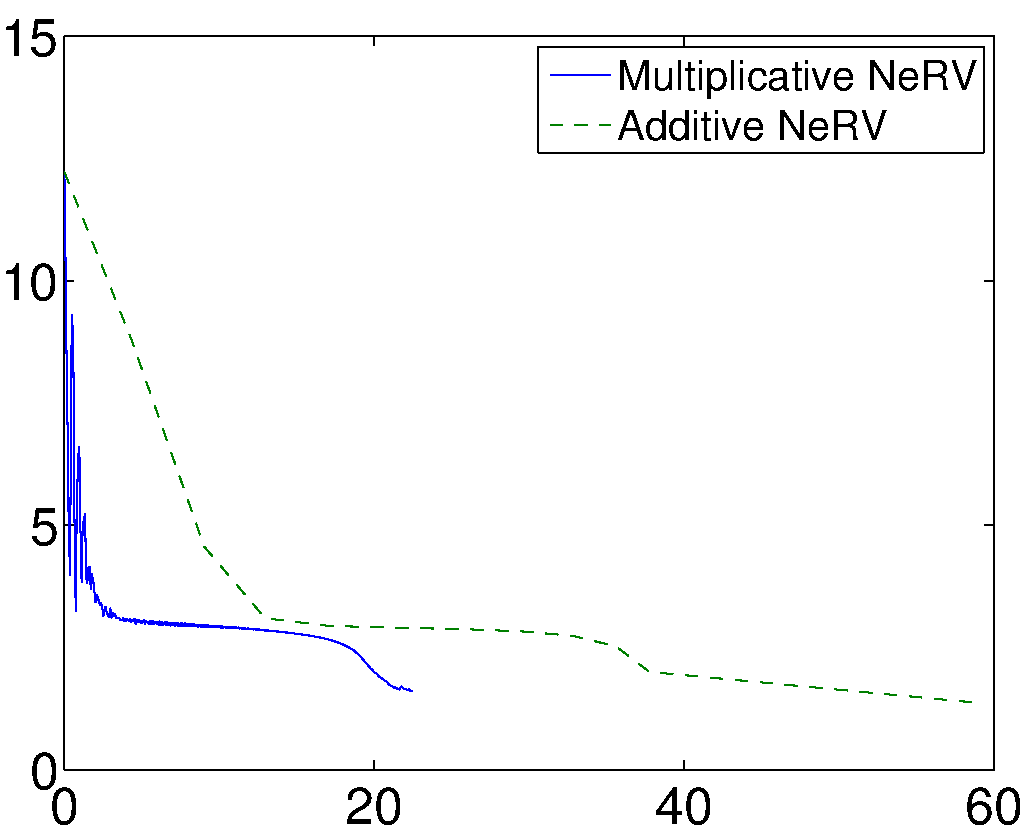
\includegraphics[width=0.5\textwidth]{figures/secs_cost_olivettifaces.pdf}} 
\end{tabular}
\caption{Graphs of running time vs. information retrieval performance (NeRV's cost, the lower the better). Data sets: MNIST and Olivetti Faces.}
\end{figure}
\end{frame}


\begin{frame}{Experiments: comparison with other NLDR methods}
\begin{figure}[!htb]
\captionsetup[subfigure]{labelformat=empty}
\centering
\begin{tabular}{cc}
\subfloat[]{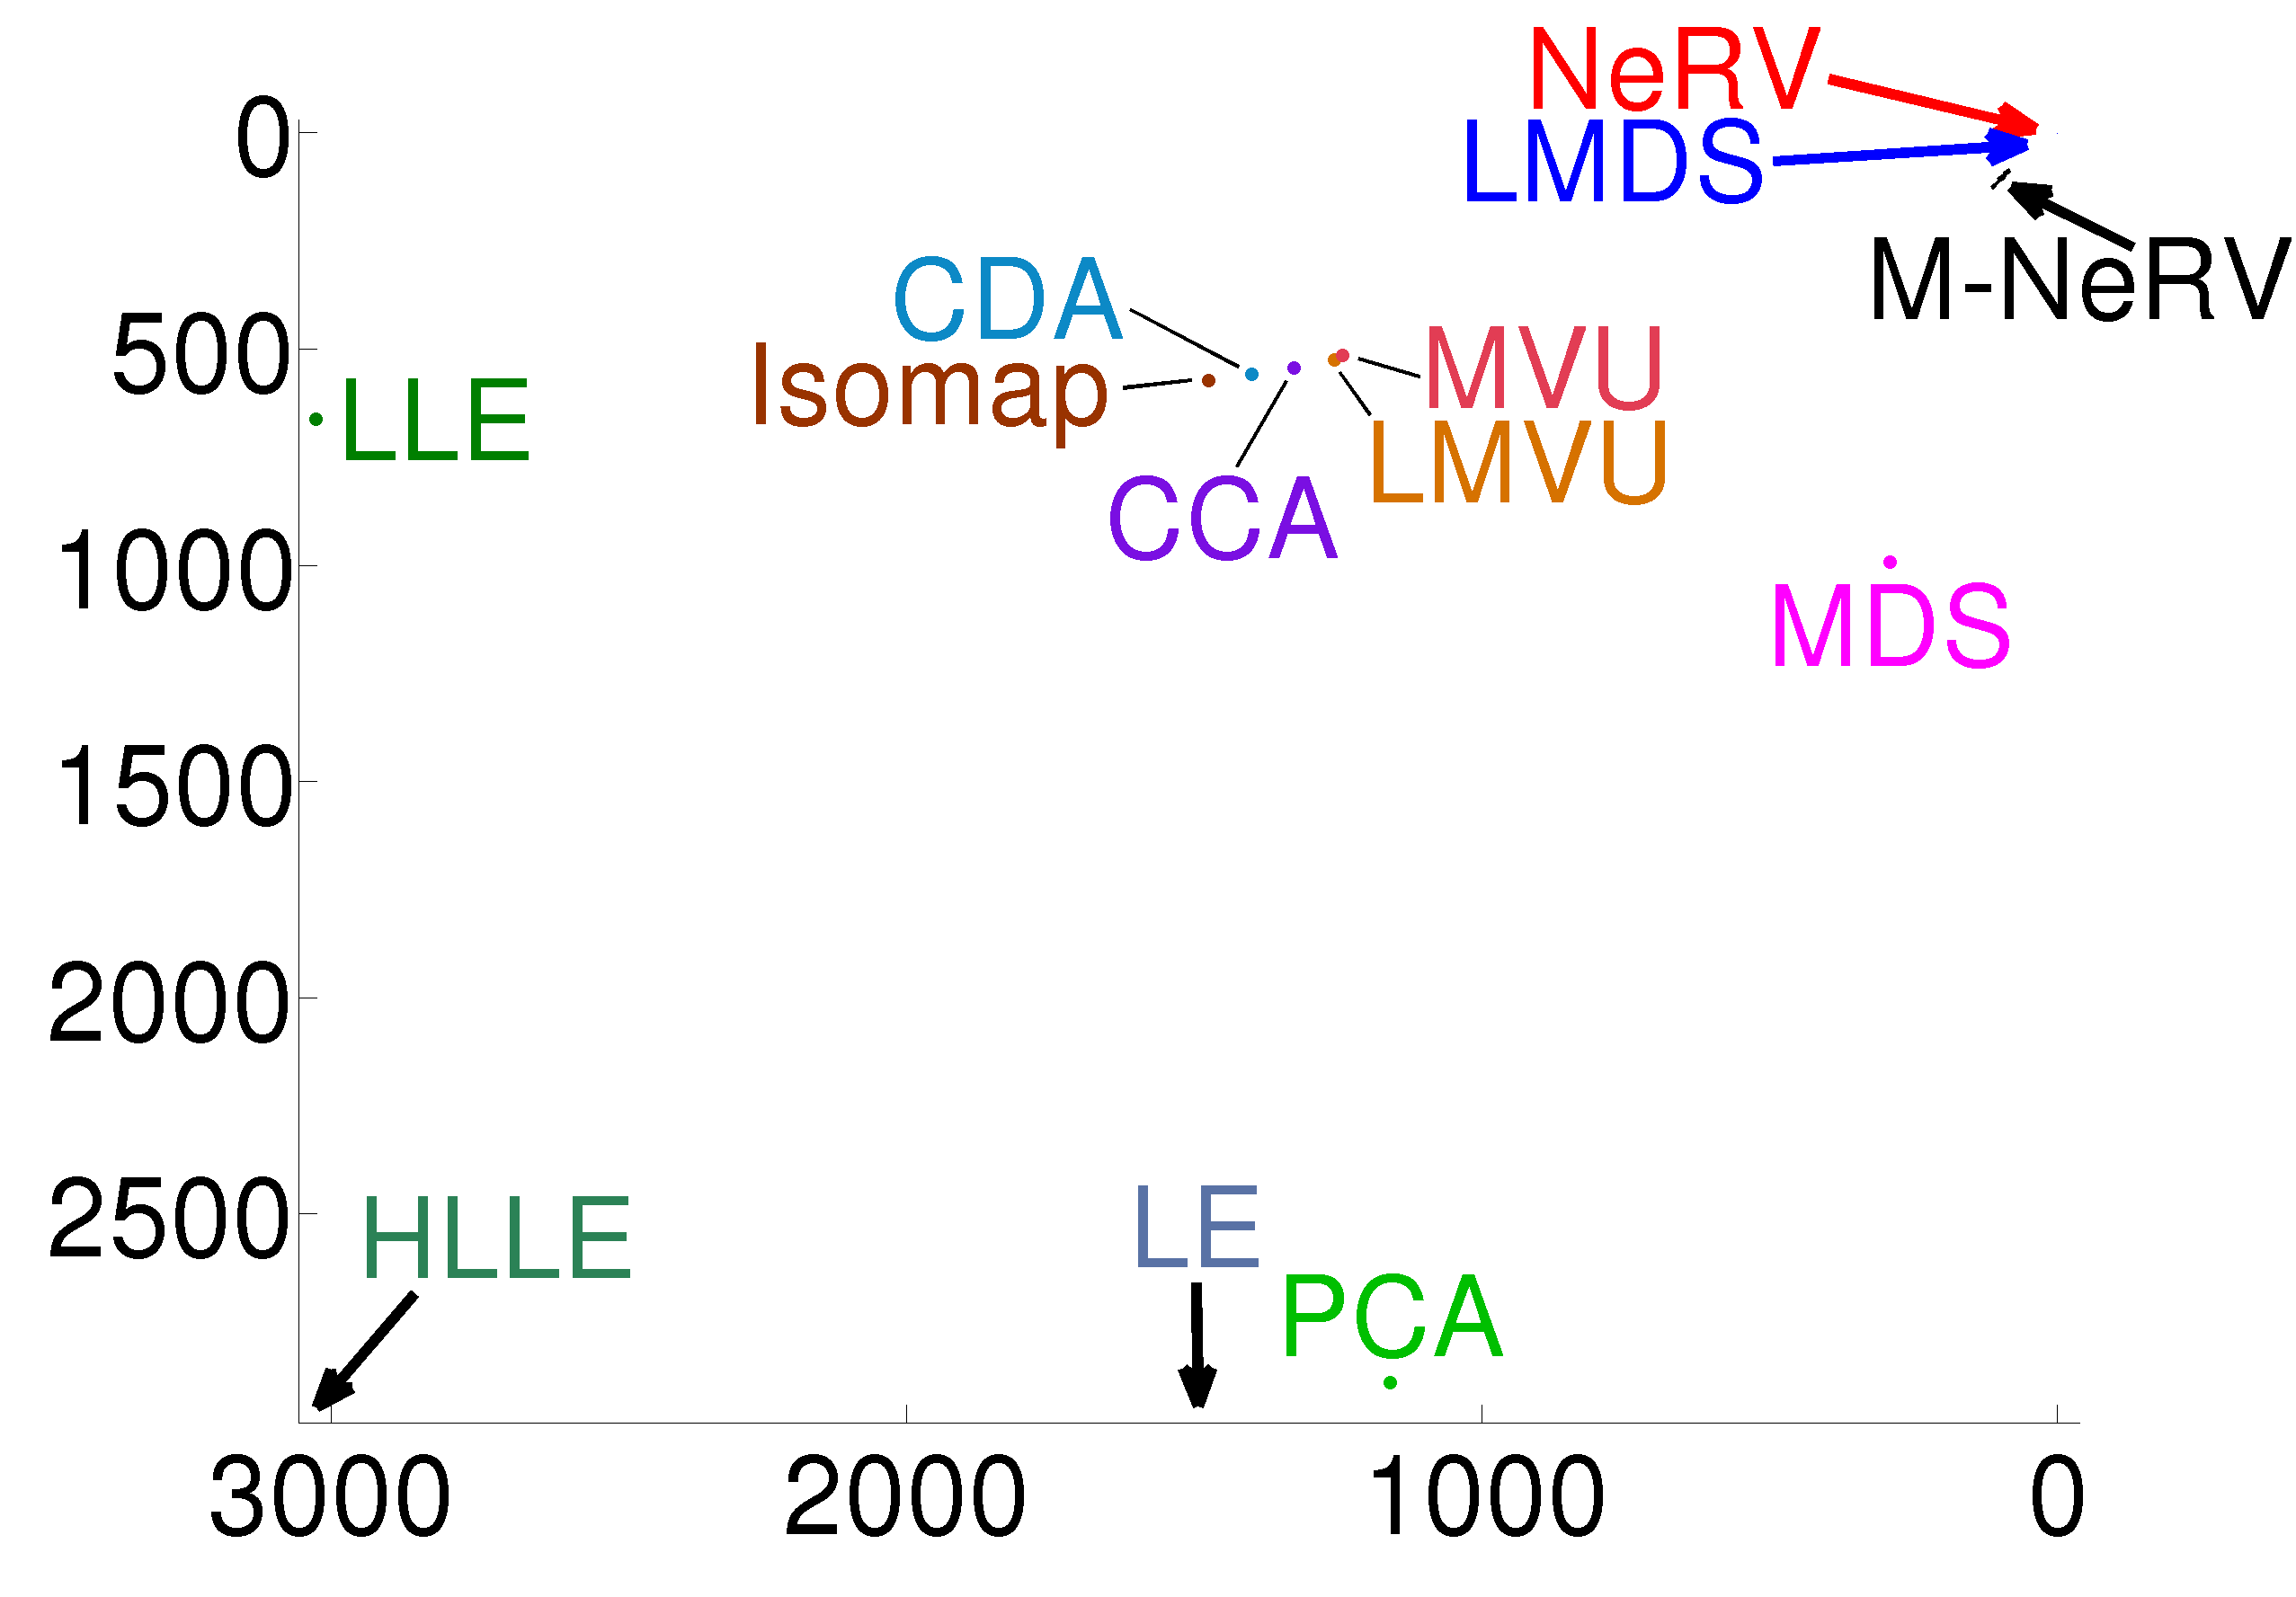
\includegraphics[width=0.5\textwidth]{figures/smoothed-precision-recall-s-data-0.pdf}} &
\subfloat[]{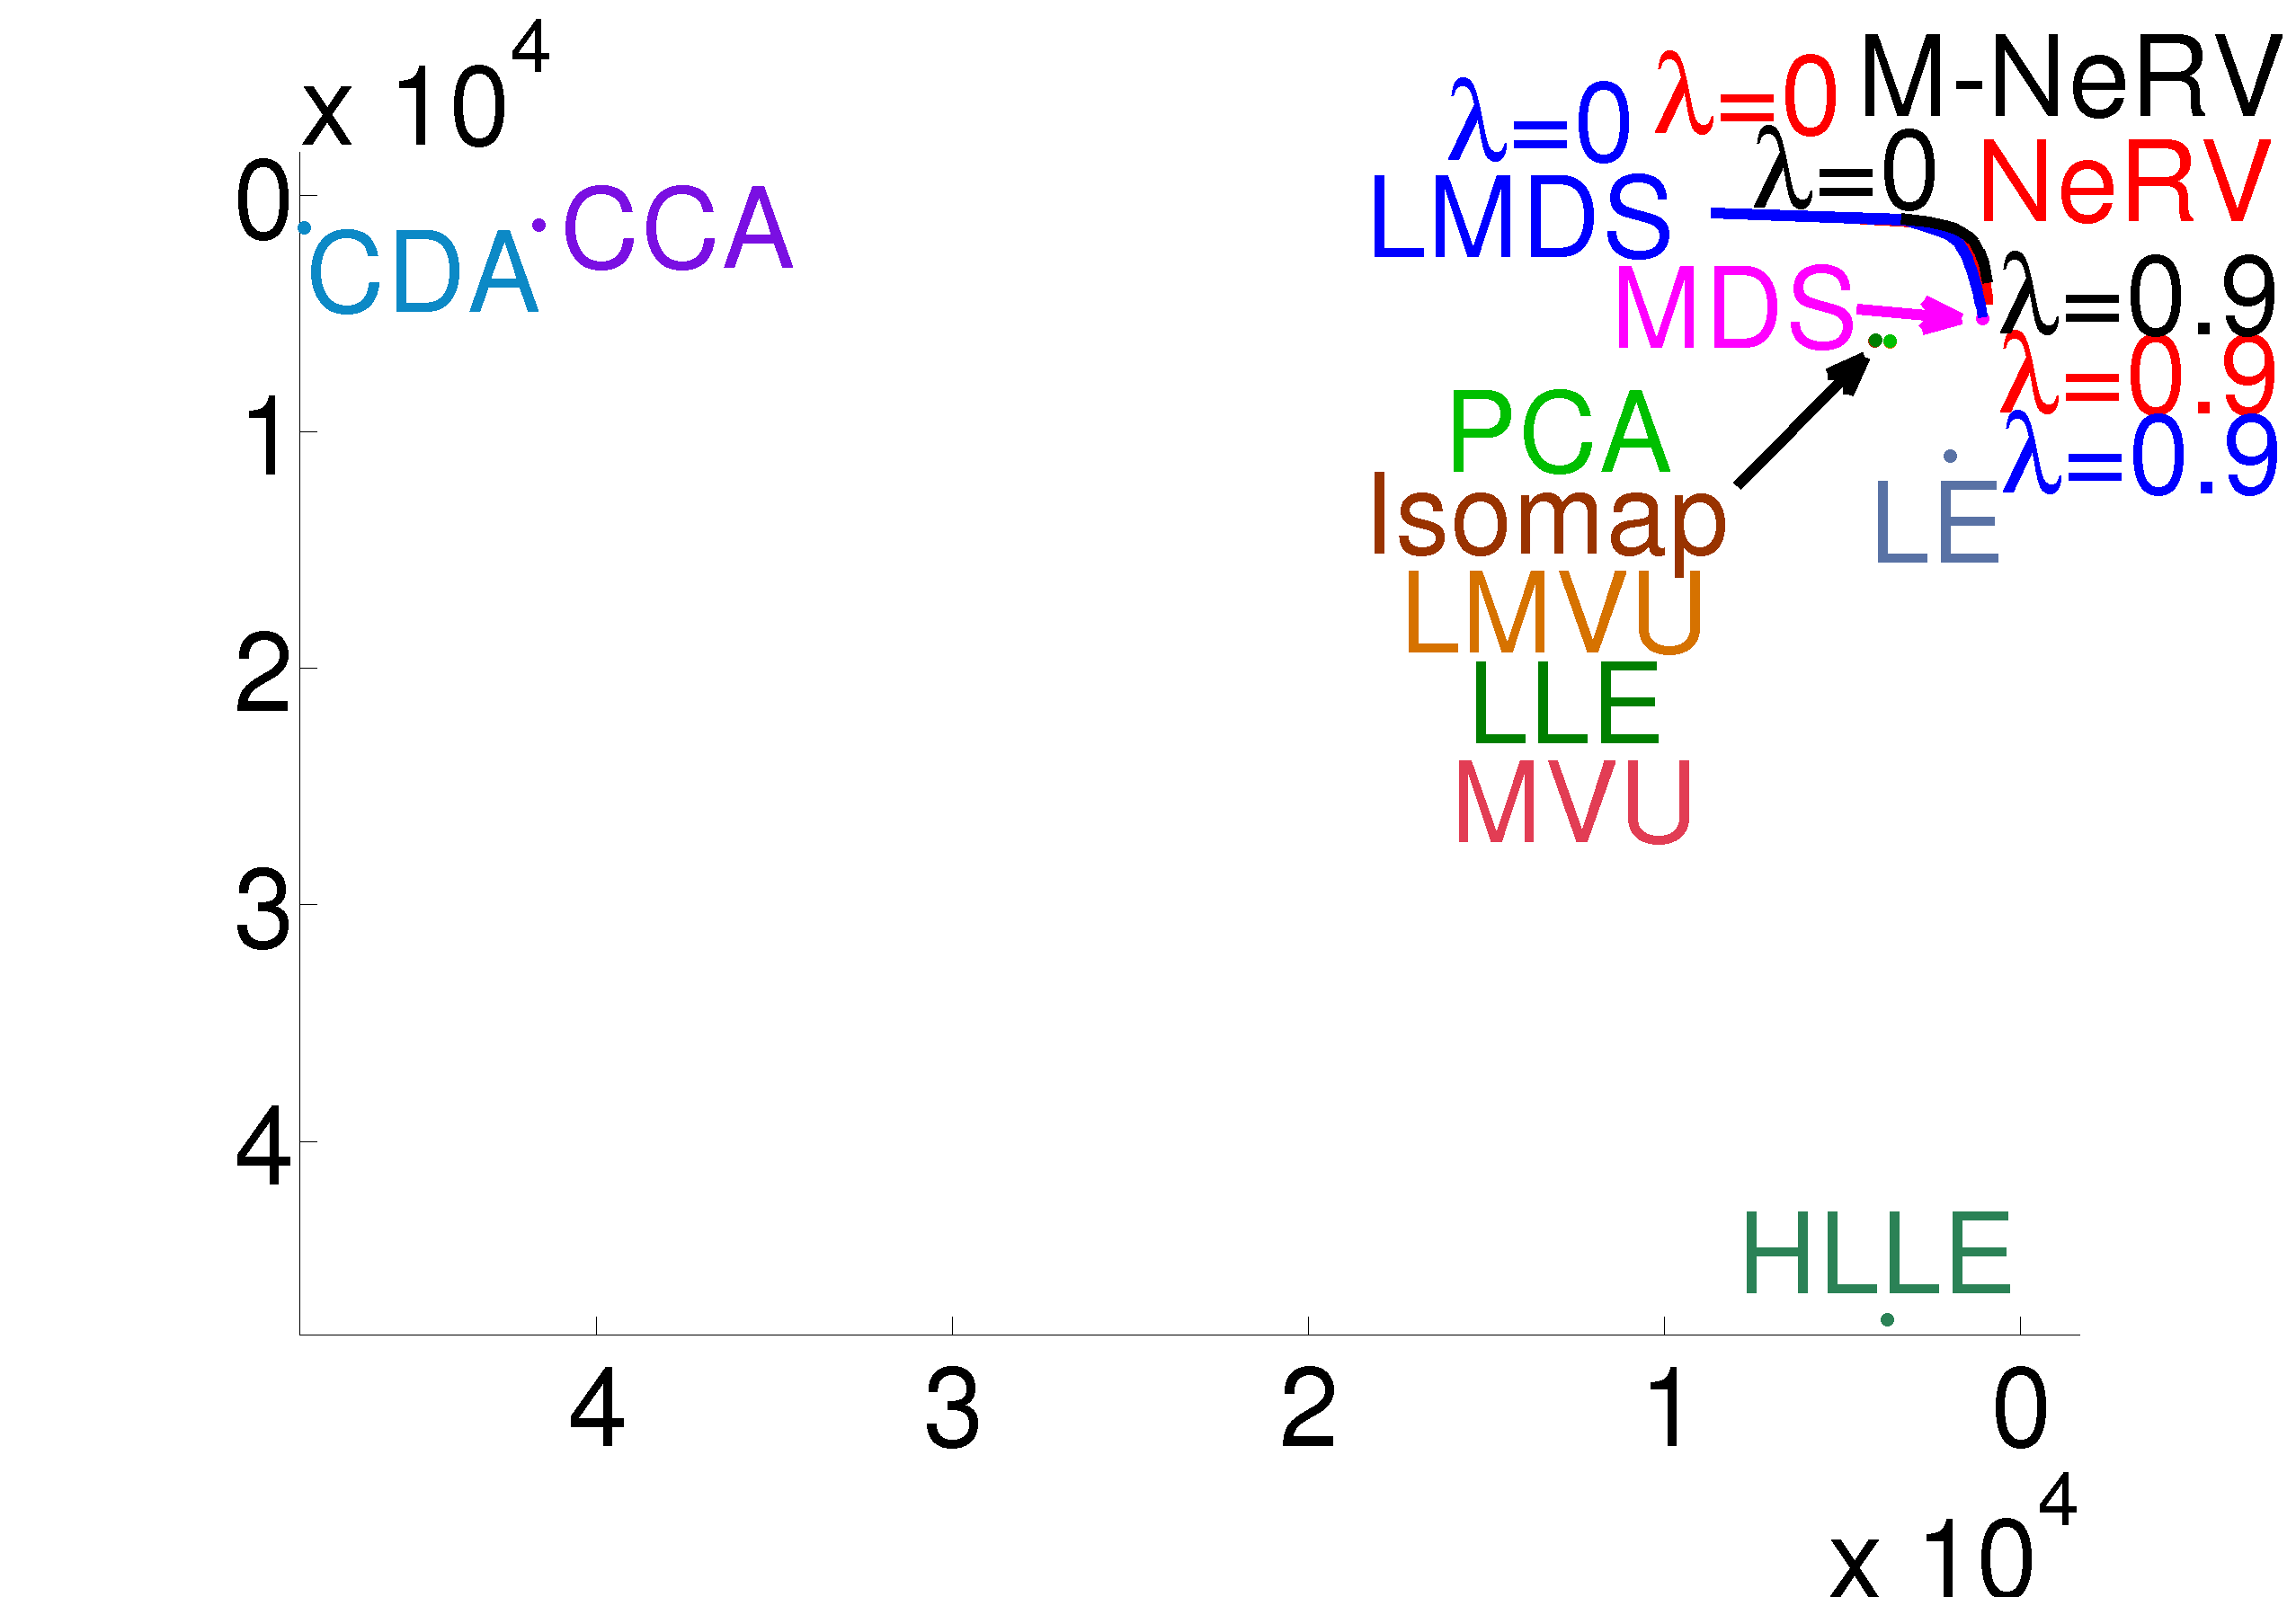
\includegraphics[width=0.5\textwidth]{figures/smoothed-precision-recall-s-data-06.pdf}} 
\end{tabular}
\caption{Mean smoothed recall vs. mean smoothed precision for different methods. Best methods locate top-right. Data sets: Plain S-curve and Noisy S-curve.}
\end{figure}
\end{frame}


\begin{frame}{Experiments: comparison with other NLDR methods}
\begin{figure}[!htb]
\captionsetup[subfigure]{labelformat=empty}
\centering
\begin{tabular}{cc}
\subfloat[]{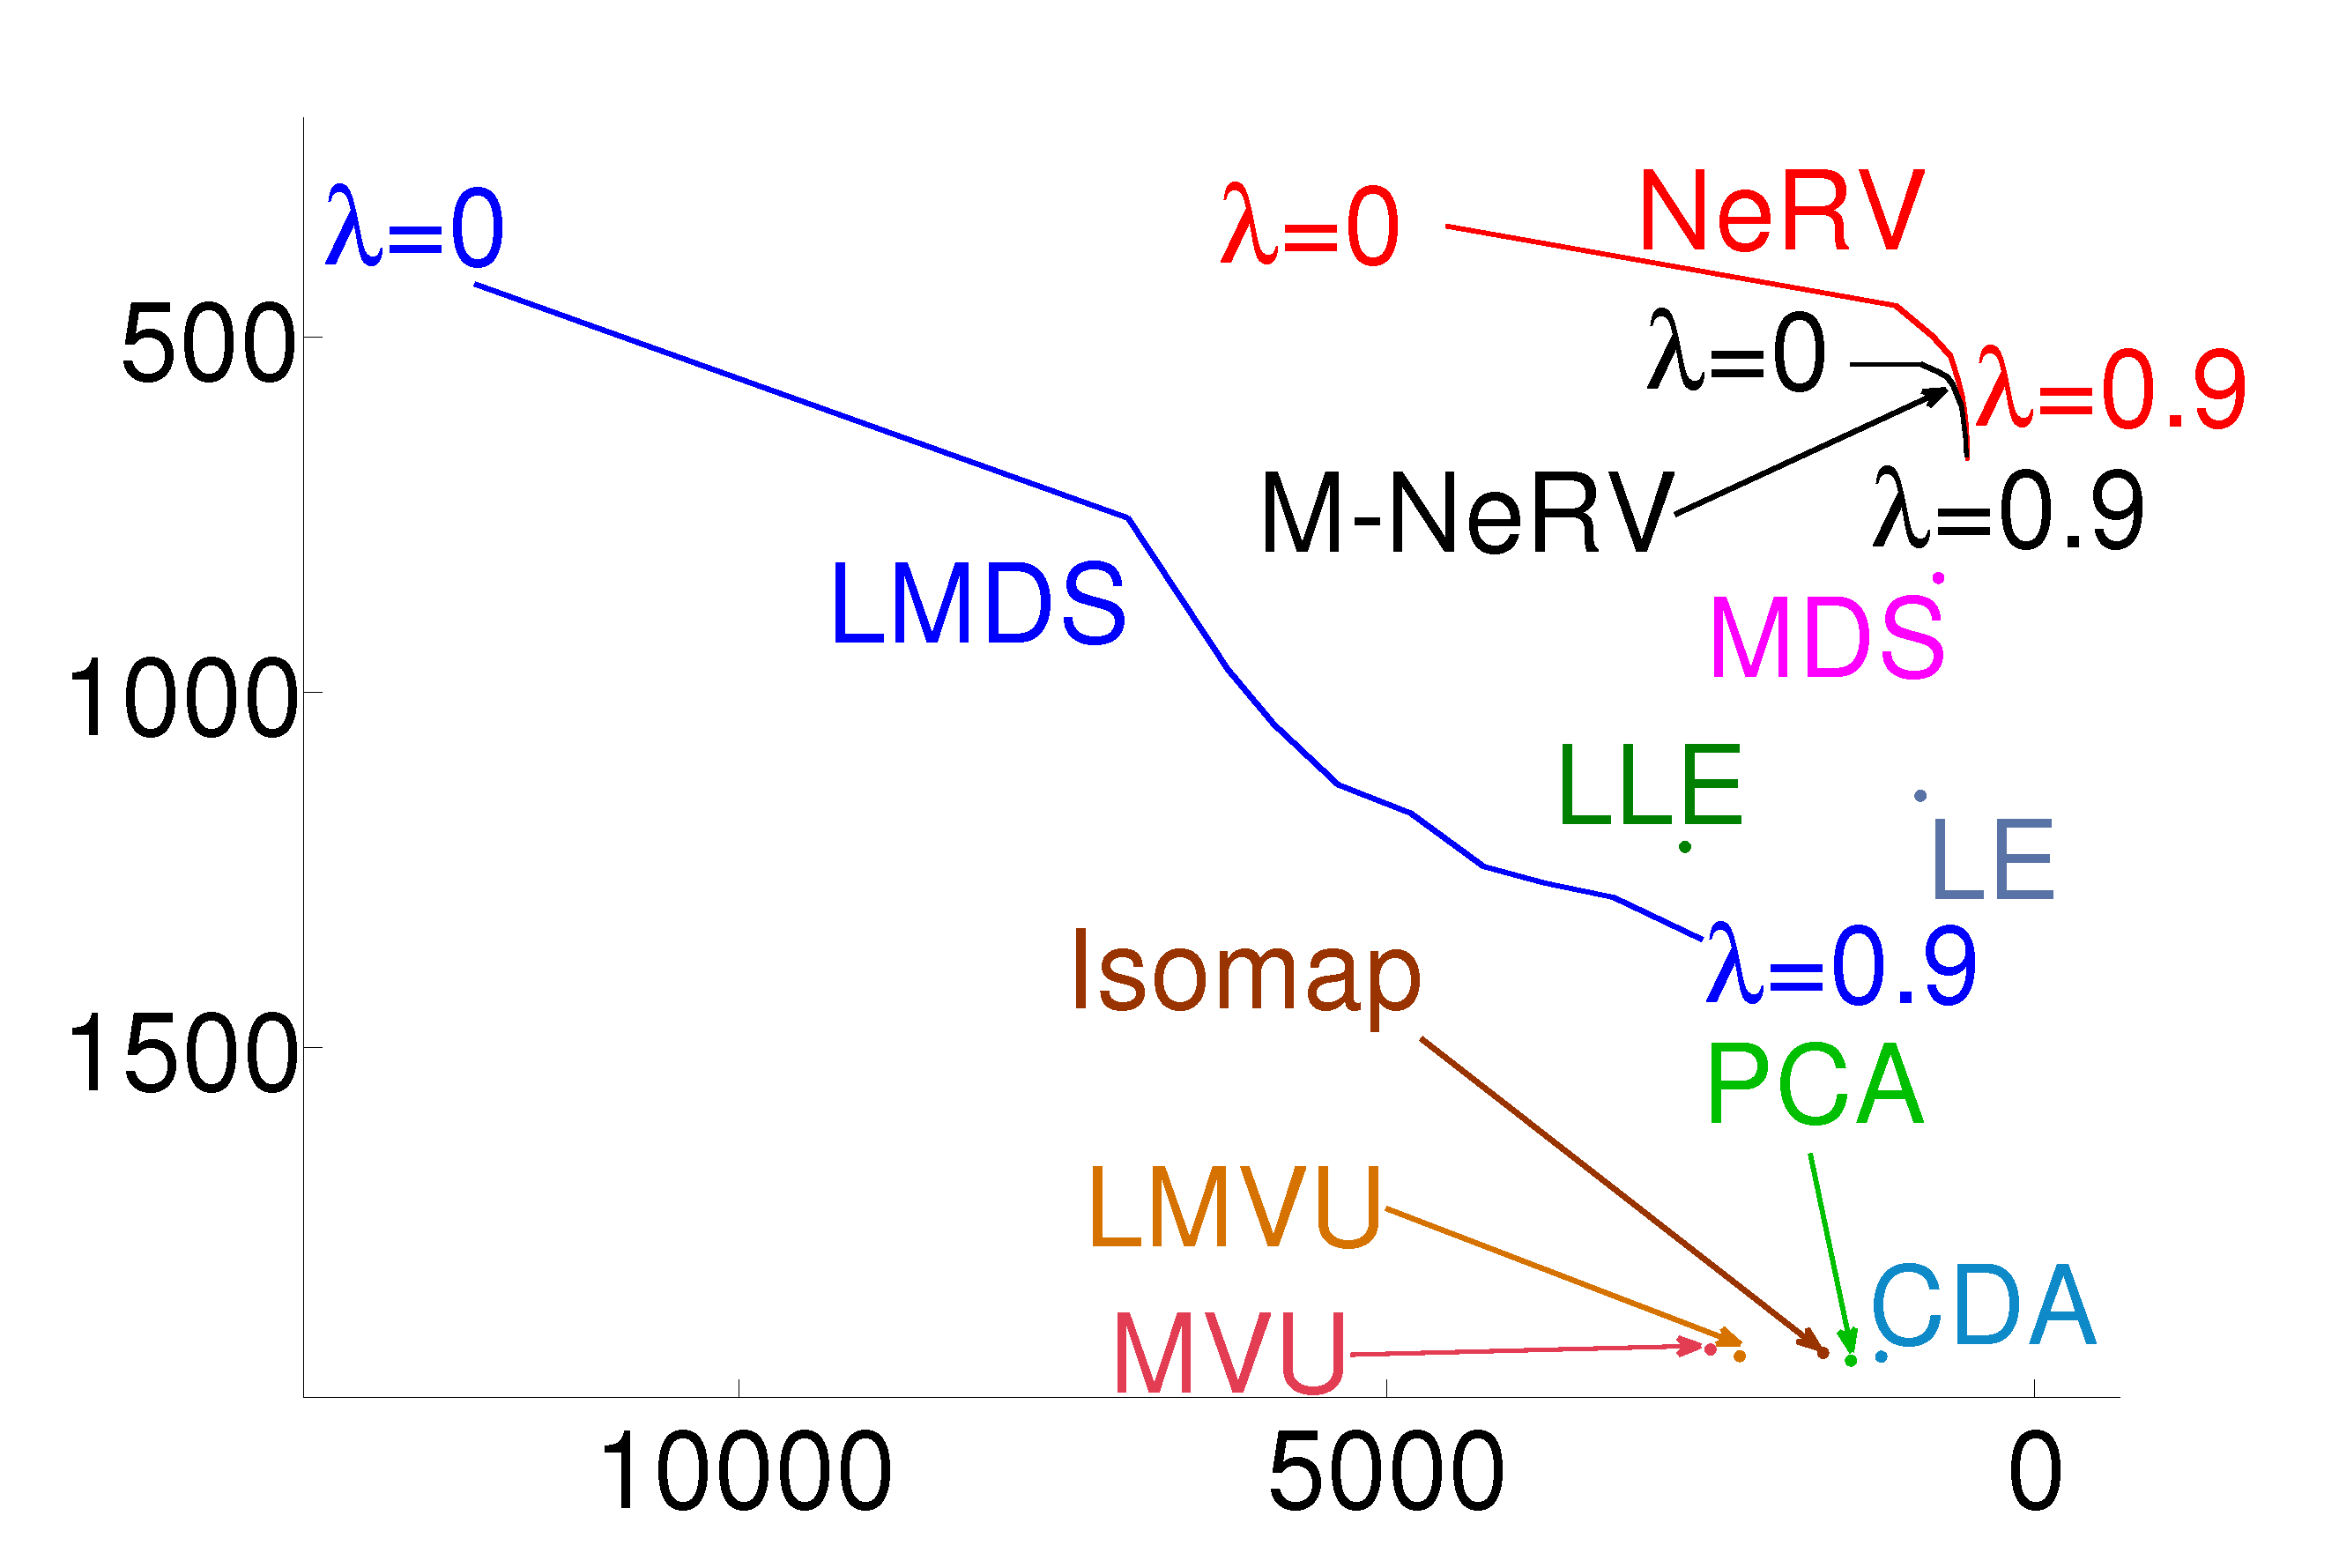
\includegraphics[width=0.5\textwidth]{figures/smoothed-precision-recall-olivettifaces.pdf}} &
\subfloat[]{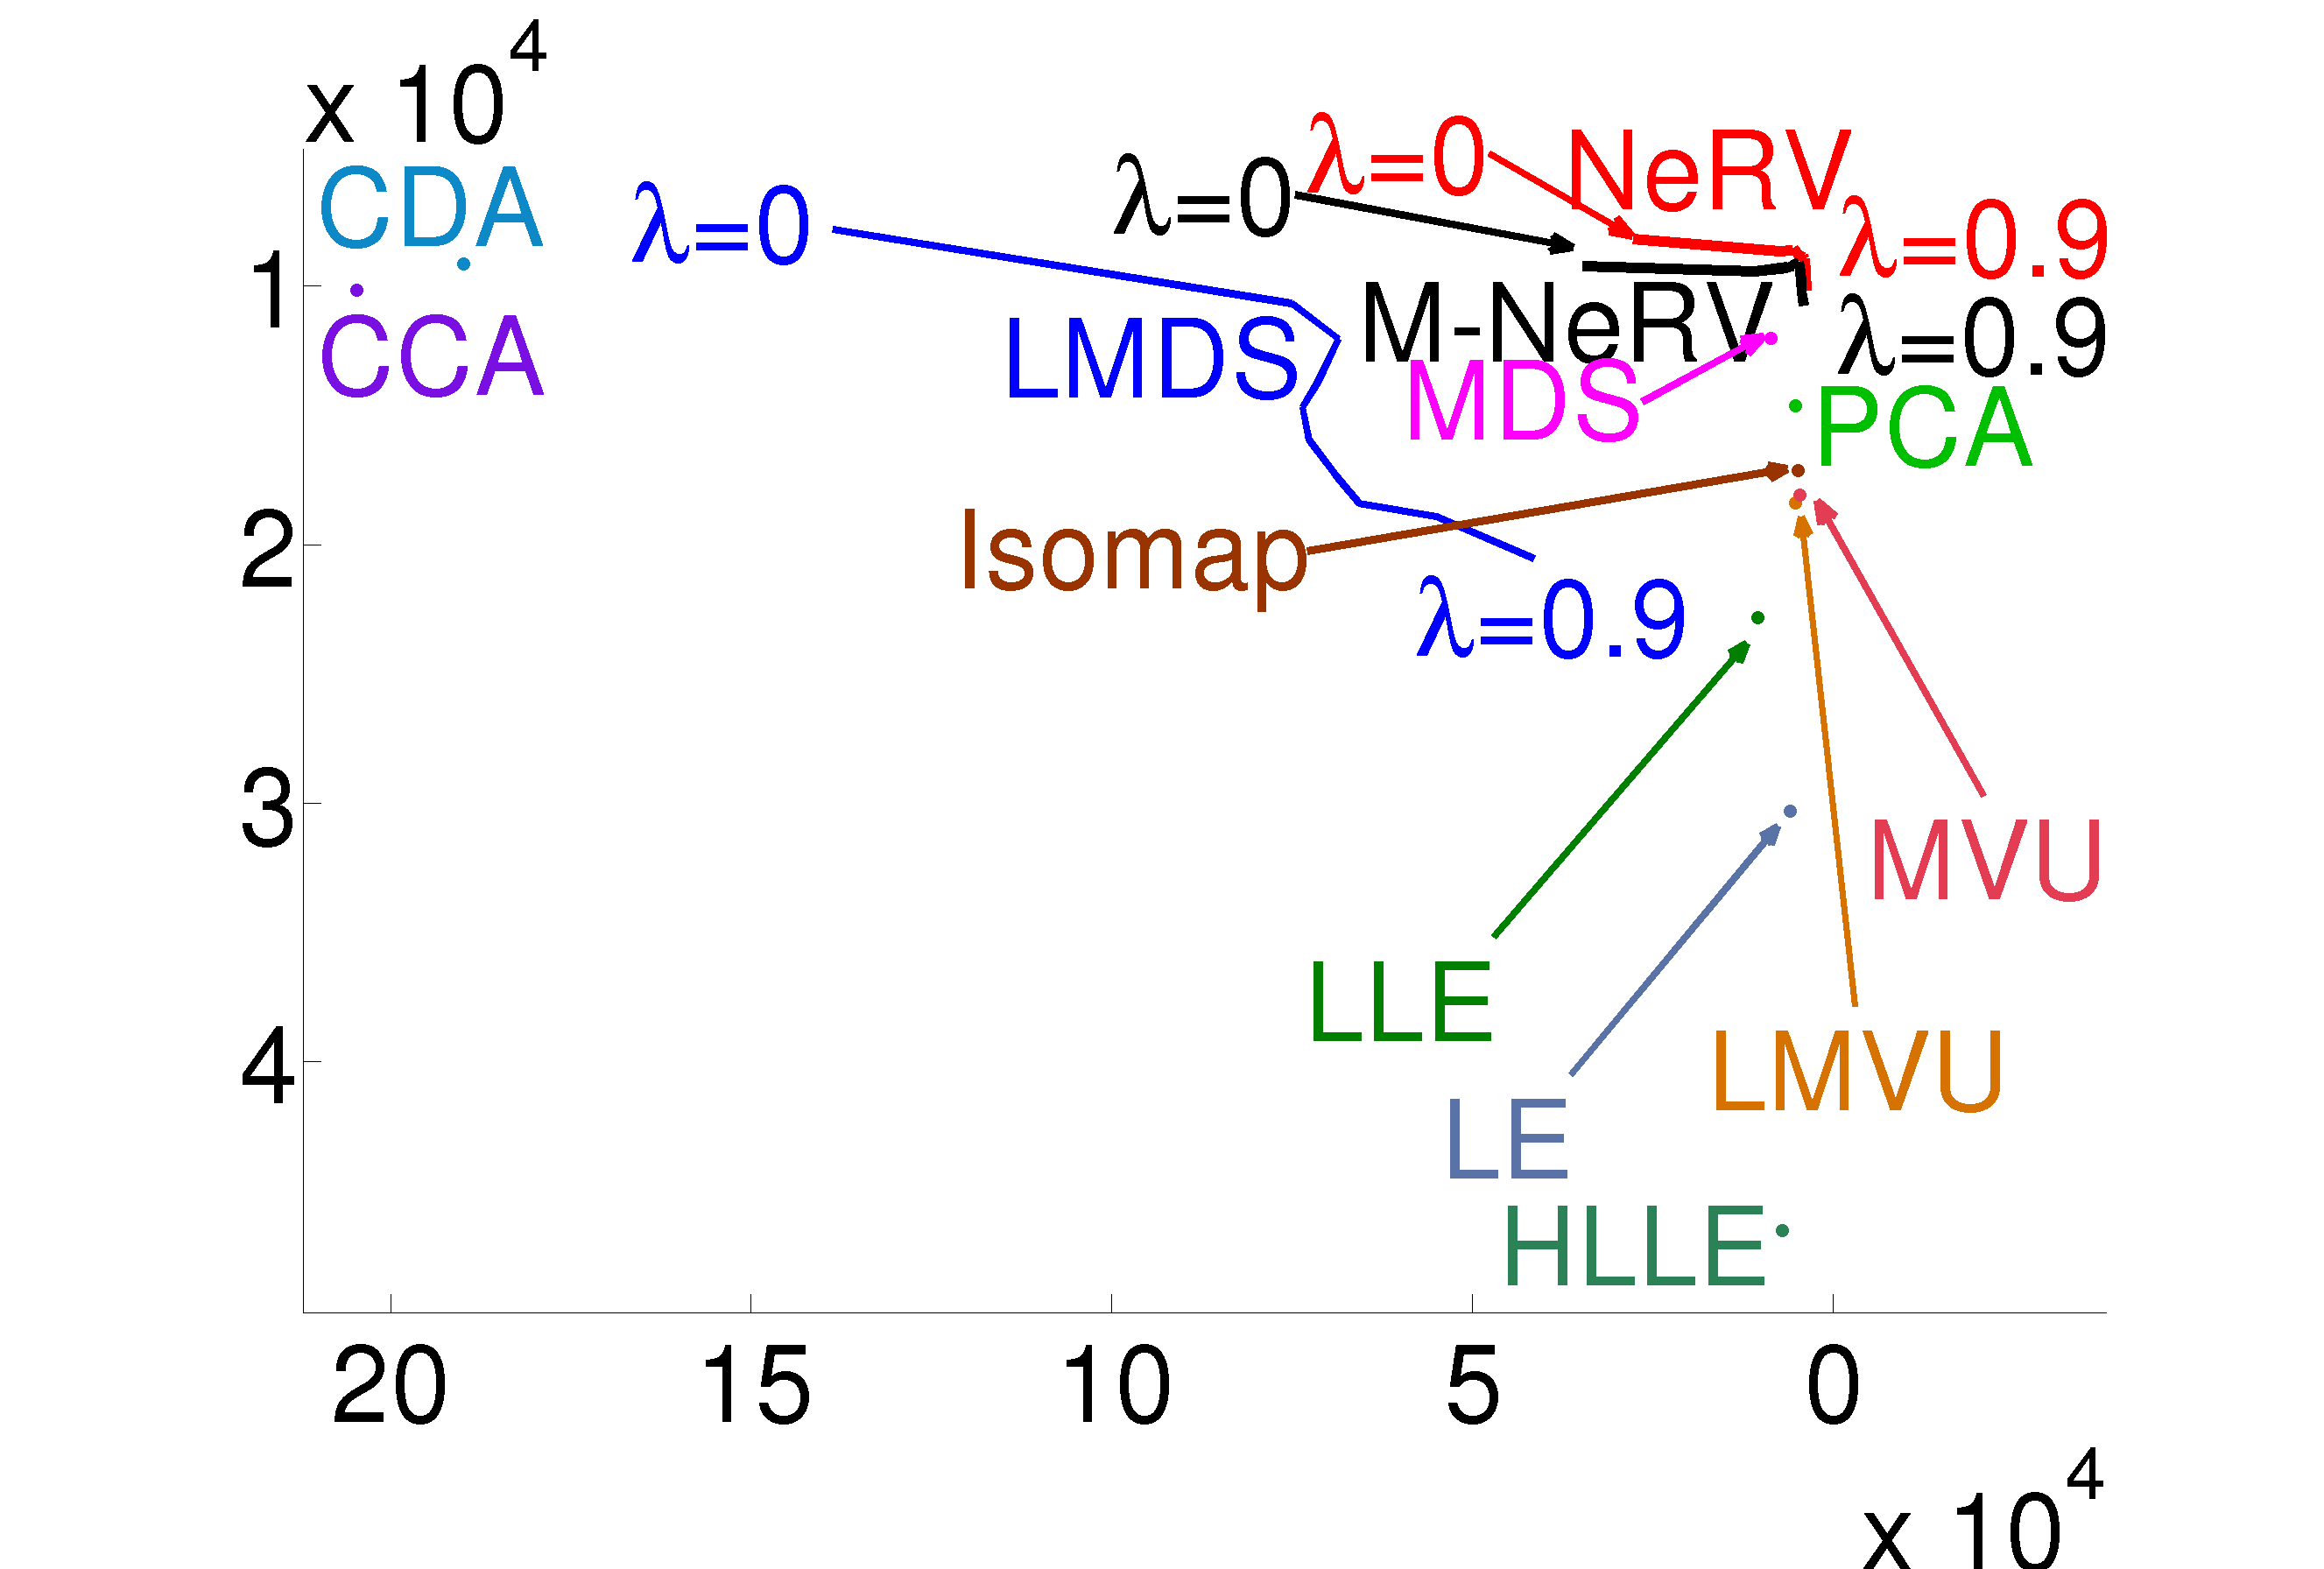
\includegraphics[width=0.5\textwidth]{figures/smoothed-precision-recall-hiiri.pdf}} 
\end{tabular}
\caption{Mean smoothed recall vs. mean smoothed precision for different methods. Best methods locate top-right. Data sets: Olivetti Faces and Mouse Gene Expression.}
\end{figure}
\end{frame}


\begin{frame}{Experiments: comparison with other NLDR methods}
\begin{figure}[!htb]
\captionsetup[subfigure]{labelformat=empty}
\centering
\begin{tabular}{cc}
\subfloat[]{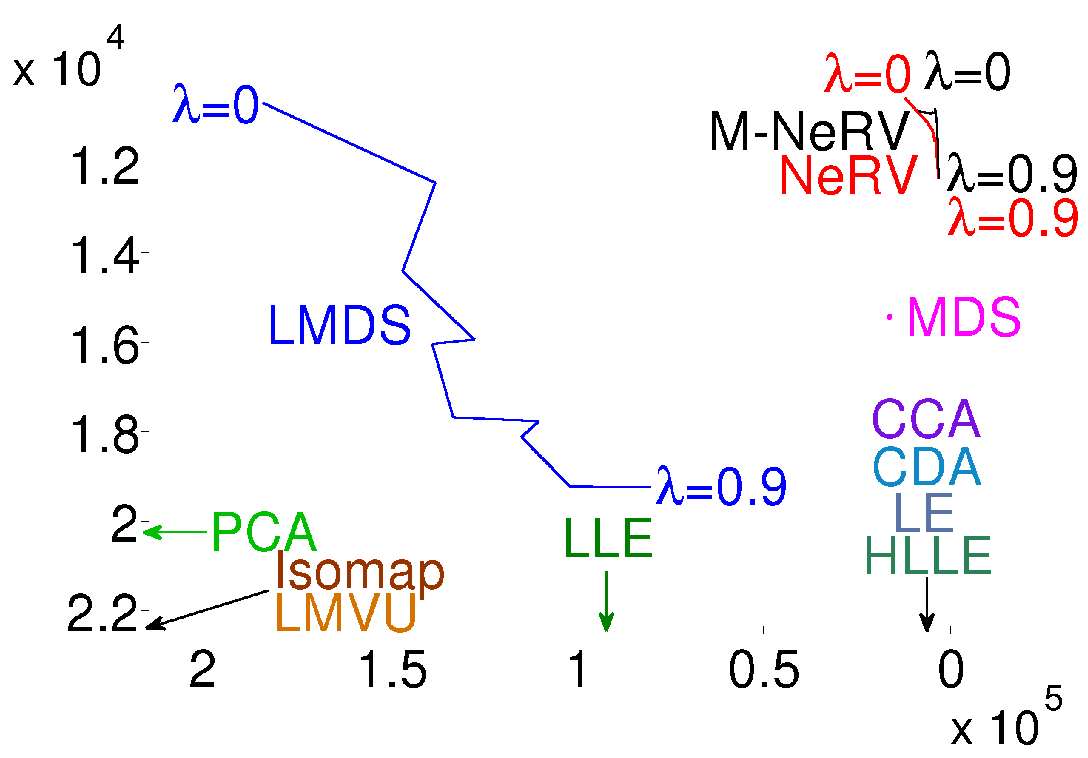
\includegraphics[width=0.5\textwidth]{figures/smoothed-precision-recall-segal-1-t.pdf}} &
\subfloat[]{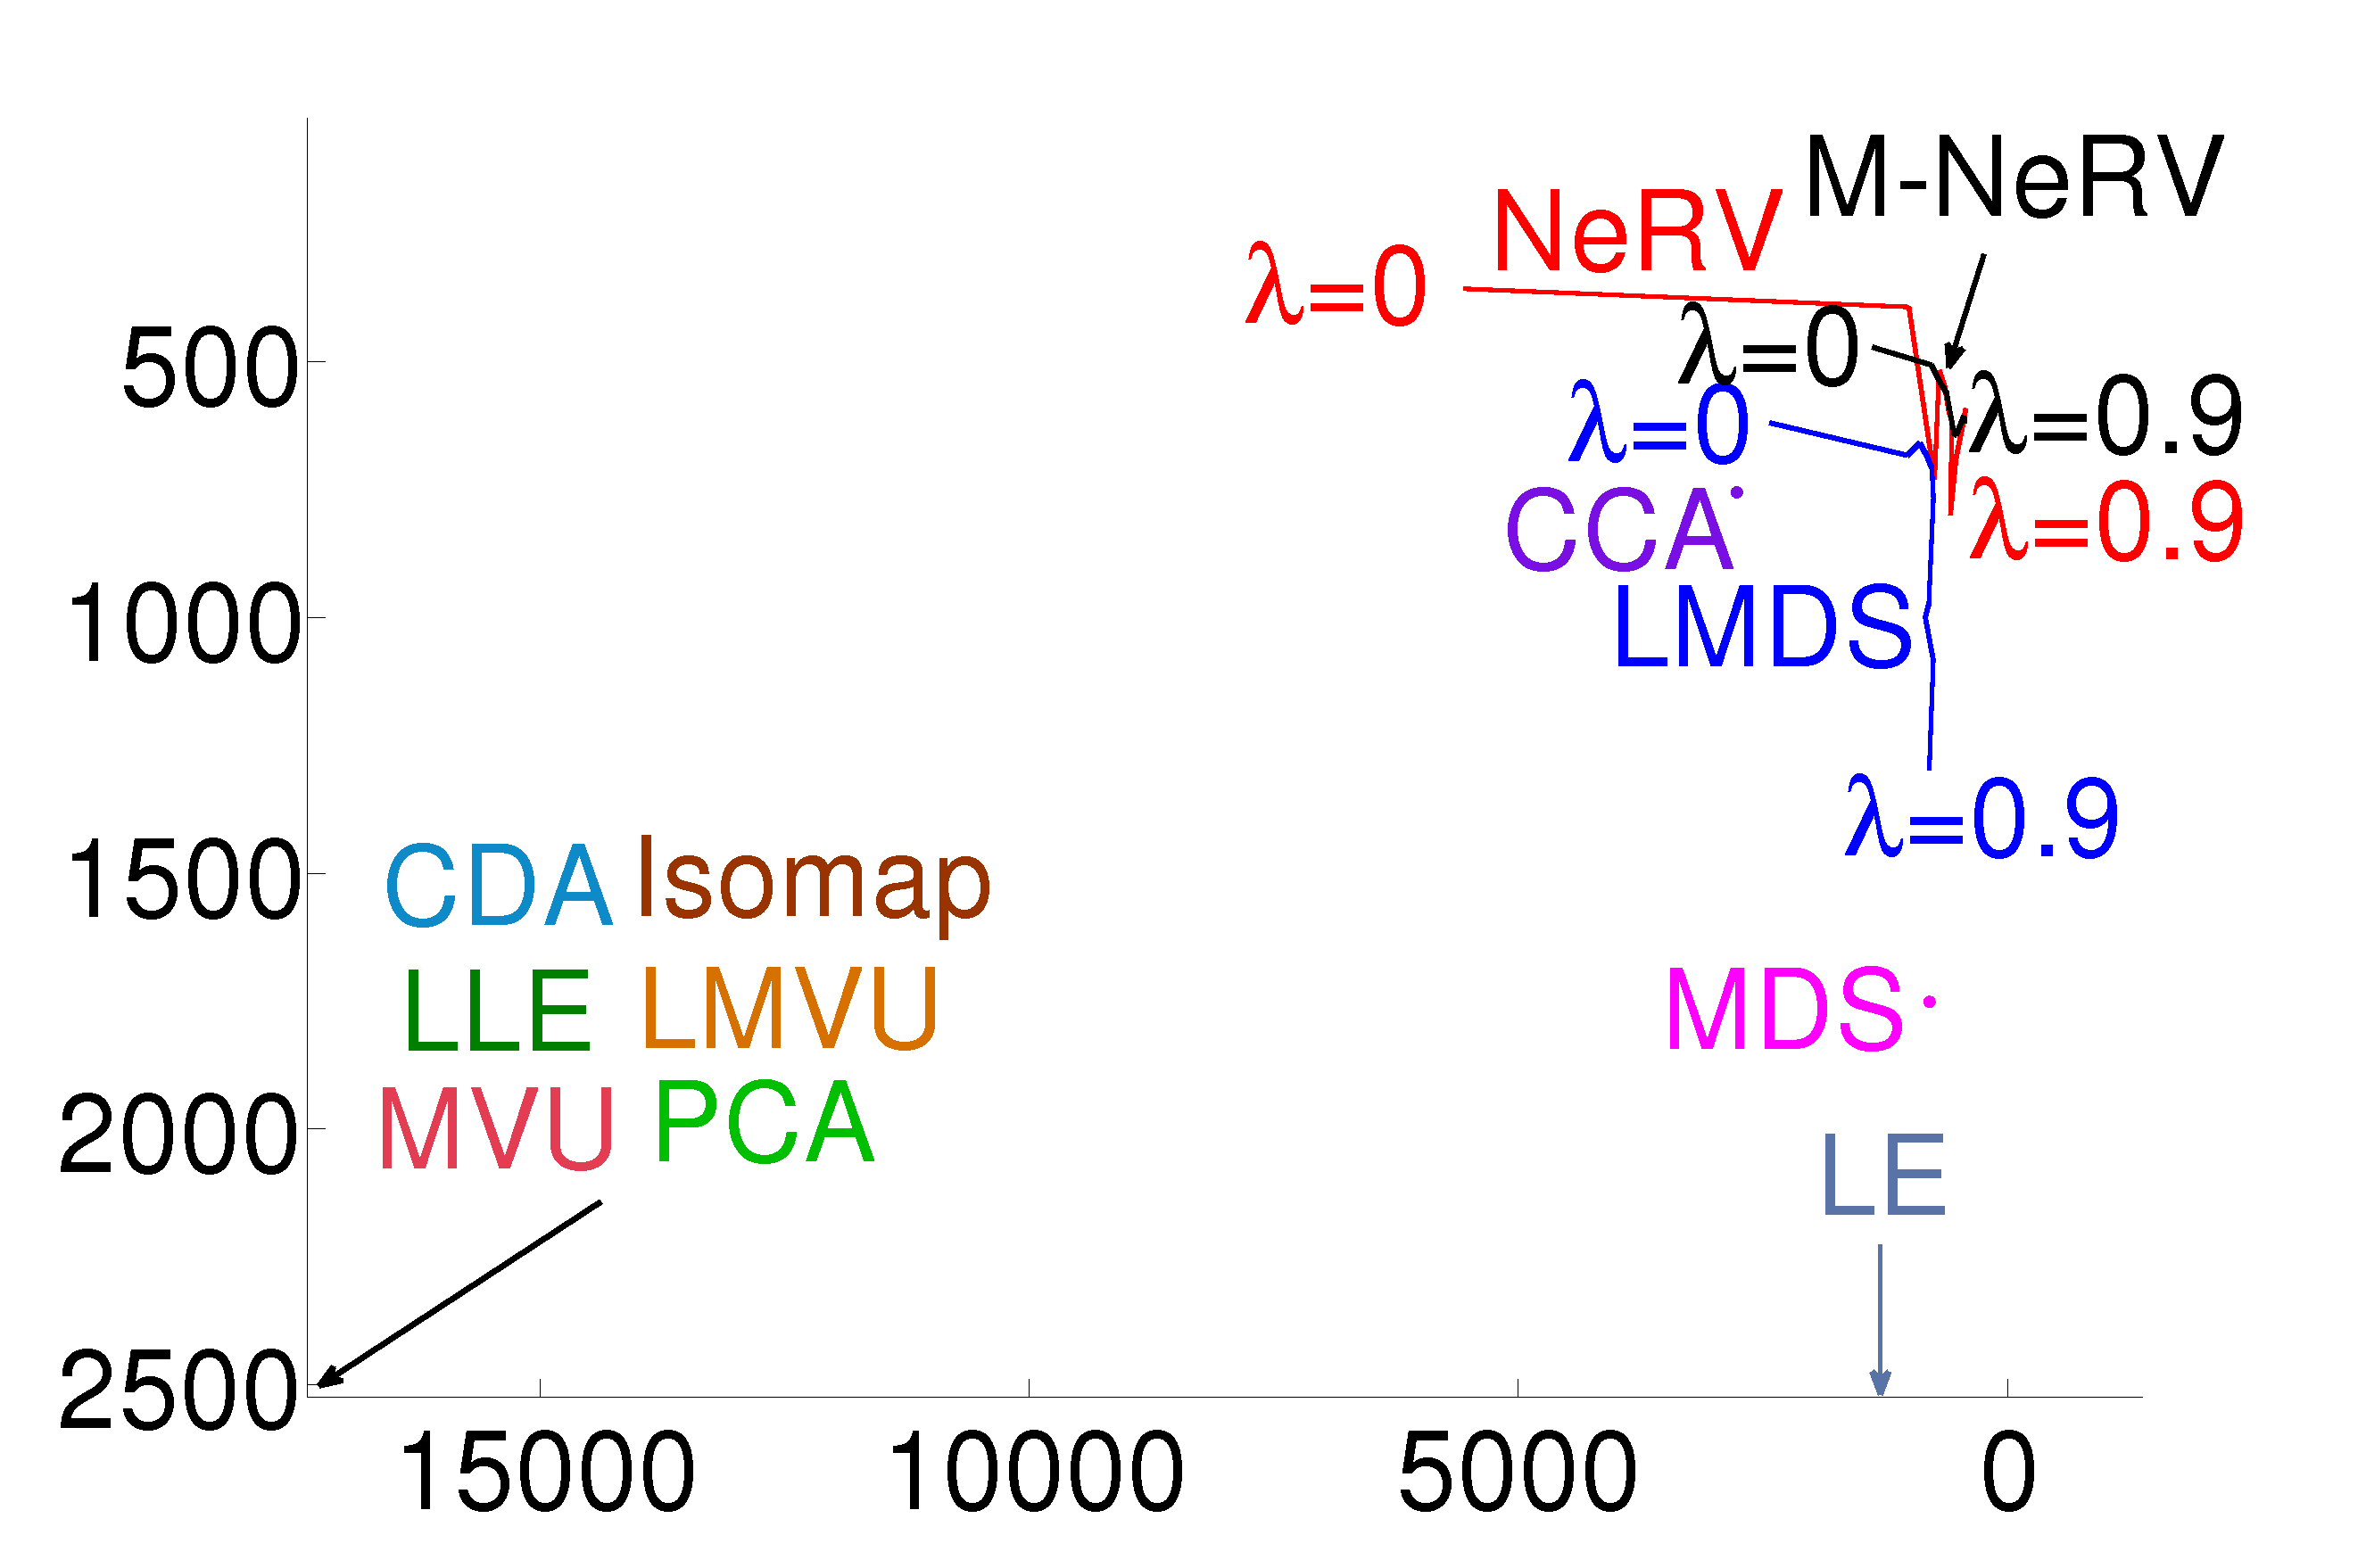
\includegraphics[width=0.5\textwidth]{figures/smoothed-precision-recall-estsp52.pdf}} 
\end{tabular}
\caption{Mean smoothed recall vs. mean smoothed precision for different methods. Best methods locate top-right. Data sets: Gene Expression Compendium and Sea-water Temperature Time Series.}
\end{figure}
\end{frame}


\begin{frame}{Conclusion}
\begin{enumerate}
\item We introduced a multiplicative update rule for the information retrieval based visualization method Neighbor Retrieval Visualizer (NeRV);
\item It needs no user-assigned learning rate parameter or line search;
\item It yields strong speedup over original NeRV and maintains state of the art performance, in terms of qualitative appearance of visualizations and quantitative information retrieval performance measures.
\end{enumerate}
\end{frame}
\end{document}